\documentclass[a4paper,11pt]{article}
\usepackage[a4paper, hmargin={3cm,2cm}, vmargin={2cm,2cm}]{geometry}
\usepackage{amsmath}
\usepackage{amsthm}
\usepackage{amsfonts}
\usepackage{color}
\usepackage[final]{graphicx}
\usepackage{subcaption}
\usepackage{wrapfig}
\newtheorem{remark}{Remark}[]
\newtheorem{prop}{Properties}
\newtheorem{theorem}{Theorem}
\usepackage{amssymb}
\usepackage{enumitem}
\usepackage{tikz}
\usepackage{smartdiagram}
\usepackage{hyperref}
\usepackage{array}

\newcommand{\R}{\mathbb{R}}
\newcommand{\C}{\mathbb{C}}
\newcommand{\N}{\mathbb{N}}
\newcommand{\Q}{\mathbb{Q}}
\newcommand{\W}{\mathbb{W}}
\newcommand{\Vspace}{\mathbb{V}}
\newcommand{\Hspace}{\mathbb{H}}
\newcommand{\Lspace}{\mathbb{L}}
\newcommand{\Lagr}{\mathcal{L}}
\newcommand{\Cmod}{\mathcal{C}}

\DeclareMathOperator*{\argmin}{argmin}

% Title Page
\title{Variational Approach to Crack Propagation\\ in a Cantilever Beam}
\author{Alifian Mahardhika Maulana}


\begin{document}
\maketitle
\section{Linear Elasticity Basic Theory}
We define:
\begin{equation*}
\begin{aligned}
&\Omega \subset \R^d\ (d=2,3)\\
&u:\Omega \rightarrow \R^d\ \text{(displacement)}\\
&e[v]:= \frac{1}{2}(\triangledown^T v + \triangledown v^T)\ \text{(strain)}\\
&\triangledown^T v := \begin{pmatrix}
\partial_1 v_1 & \partial_2 v_2\\
\partial_1 v_2 & \partial_2 v_1
\end{pmatrix}\\
& \triangledown v^T := ( \triangledown^T v)^T\\
&\sigma[u]:=\Cmod e[u]\\
&\Cmod=(C_{ijkl})\begin{cases}
C_{ijkl}=C_{klij}=C_{jikl}\\
(C_\xi):\xi \geq C_* |\xi|^2 (\forall \xi \in \R_{sym}^{d\times d})
\end{cases}
\end{aligned}
\end{equation*}
Let's consider linear elasticity problem:
\begin{equation}\label{eq:stronglinear}
(**)\begin{cases}
-div\ \sigma[u]=f(x),\ \text{in}\ \Omega\\
u=g(x)\ \text{on}\ \Gamma_D\\
\sigma[u] \nu = q(x)\ \text{on}\ \Gamma_N
\end{cases}
\end{equation}
\begin{equation*}
f \in L^2(\Omega : \R^d,\ g\in H^1(\Omega : \R^d),\ q\in L^2(\Gamma_N:\R^d))
\end{equation*}
\subsection{Strong Solution}
\begin{equation}
u\in H^2 (\Omega : \R^d)\ \text{satisfies}\ (**)\ \text{then we call $u:$ a strong solution}
\end{equation}
\subsection{Weak Solution}
\begin{equation}\label{eq:weaklinear}
\begin{cases}
\int_\Omega \sigma[u] : e[v] dx = \int_\Omega f\cdot v dx + \int_{\Gamma_N} q\cdot v ds \big( \forall v \in V:= \{ v \in H^1\ (\Omega : \R^d)\ |v|_{\Gamma_D} = 0 \}\big)\\
u \in V+g
\end{cases}
\end{equation}
\subsection{Proposition}
\begin{equation*}
u:\ \text{strong solution}\ \Leftrightarrow \begin{cases}
u:\ \text{weak solution}\\
u\in H^2\ (\Omega : \R^d)
\end{cases}
\end{equation*}
\begin{proof}
	($\Rightarrow$)
	Assume we choose $v \in V:= \{ v \in H^1\ (\Omega : \R^d)\ |v|_{\Gamma_D} = 0 \}$, with $v$ is a very smooth test function. Then we take integral over the domain for equation \eqref{eq:stronglinear} on both side.
	\begin{equation*}
	\begin{aligned}[center]
	\int_\Omega -div\sigma[u] \cdot v dx &= \int_\Omega f \cdot v dx\\
	\int_\Omega \sigma[u] : \triangledown v dx - \int_\Gamma \sigma[u]\nu \cdot v ds &= \int_\Omega f \cdot v dx\  \text{(by Divergence Formula)}\\
	\int_\Omega \sigma[u] : \triangledown v dx - \bigg(\int_{\Gamma_D} \sigma[u]\nu \cdot v ds + \int_{\Gamma_N} \sigma[u]\nu \cdot v ds\bigg) &= \int_\Omega f \cdot v dx\\	
	\end{aligned}
	\end{equation*}
	From Boundary Condition we know that:
	\begin{equation*}
	\begin{cases}
	v = 0\ \text{on}\ \Gamma_D\\
	\sigma[u] \nu = q\ \text{on}\ \Gamma_N
	\end{cases}
	\end{equation*}
	Hence, we have:
	\begin{equation}\label{weakproof}
	\begin{aligned}[center]
	\int_\Omega \sigma[u] : e[v] dx - \int_{\Gamma_N} q \cdot v ds &= \int_\Omega f \cdot v dx\\
	\int_\Omega \sigma[u] : e[v] dx &= \int_\Omega f \cdot v dx + \int_{\Gamma_N} q \cdot v ds \\
	\end{aligned}
	\end{equation}
	with:
	\begin{equation*}
	\begin{aligned}
	&X:= H^1(\Omega : \R^d)\\
	&a(u,v) := \int_\Omega \sigma[u] : e[v] dx\\
	&l(v) := \int_\Omega f\cdot v dx + \int_{\Gamma_N} q \cdot v ds\\
	\end{aligned}
	\begin{aligned}
	a(u,v) &= \int_\Omega (\Cmod e[u]) : e[v] dx\\
	&= \int_\Omega e[v] : (\Cmod e[u]) dx\\
	&= a(v,u)
	\end{aligned}
	\end{equation*}
	Then we rewrite equation \eqref{weakproof} in a bilinear and linear form:
	\begin{equation*}
	a(u,v) = l(v)
	\end{equation*}
	
	($\Leftarrow$)
	Since $u\in H^2\ (\Omega : \R^2), div(\sigma[u]) \in L^2(\Omega: \R^2)$ and $a(u,v)=0$ for all $v \in V$, we have:
	\begin{equation*}
	\begin{aligned}[center]
	0 &= \int_\Omega \sigma[u] : e[v] dx\\
	0 &= \int_\Omega \begin{pmatrix}
	\sigma_{11} & \sigma_{12}\\
	\sigma_{21} & \sigma_{22}\\
	\end{pmatrix} : \begin{pmatrix}
	\triangledown v_1 & \triangledown v_2
	\end{pmatrix} dx\\
	0 &= \int_\Omega \begin{pmatrix}
	\sigma_{11}\\
	\sigma_{21}
	\end{pmatrix} \cdot \triangledown v_1 + \begin{pmatrix}
	\sigma_{12}\\
	\sigma_{22}
	\end{pmatrix} \cdot \triangledown v_2 dx\\
	0 &= \int_\Omega div \begin{pmatrix}
	\sigma_{11}\\
	\sigma_{21}
	\end{pmatrix} v_1 + div \begin{pmatrix}
	\sigma_{12}\\
	\sigma_{22}
	\end{pmatrix} v_2 - \int_{\partial\Omega} \begin{pmatrix}
	\sigma_{11}\\
	\sigma_{21}
	\end{pmatrix} \cdot \nu v_1 + \begin{pmatrix}
	\sigma_{12}\\
	\sigma_{22}
	\end{pmatrix} \cdot \nu v_2 ds\\
	0 &= \int_\Omega (f + div \sigma[u]) \cdot v dx - \int_{\partial\Omega} (\sigma[u]\nu)\cdot v ds\\
	0 &= \int_\Omega f \cdot v dx + \int_\Omega div \sigma[u] \cdot v dx - \int_{\partial\Omega} (\sigma[u]\nu)\cdot v ds
	\end{aligned}
	\end{equation*}
	then, assume we choose $v \in C_0^\infty (\Omega) \subset V, v = 0\ \text{near}\ \partial\Omega$\\
	$f \in L^1(\Omega),$ then we have:
	\begin{equation*}
	\begin{aligned}[center]
	\int_\Omega (f + div \sigma[u]) \cdot v dx &= 0\ (\forall v \in C_0^\infty(\Omega,\R^2))\\
	\therefore f + div \sigma[u] &= 0\ \text{in}\ \Omega
	\end{aligned}
	\end{equation*}
	then, $\forall v \in C_0^\infty (\bar{\Omega})$ s.t. $(supp(v) \cap \partial\Omega) \subset \Gamma_N$
	\begin{equation*}
	\begin{aligned}[center]
	\int_{\Gamma_N} (\sigma[u]\nu)\cdot v ds &= 0\\
	\sigma[u]\nu &= 0\ \text{on}\ \Gamma_N
	\end{aligned}
	\end{equation*}
\end{proof}
For $v \in V$
\begin{equation*}
\begin{aligned}
a(v,v) &= \int_\Omega (\Cmod e[v]) : e[v] dx\\
&\geqq C_* \int_\Omega |e[v]|^2 dx\\
&\geqq C_* ||v||^2_x
\end{aligned}
\end{equation*}
\begin{prop}
	\begin{itemize}
		\item $a(\cdot,\cdot)$ is bounded symmetric, bilinear form on $X \times X$.
		\item $a(\cdot,\cdot)$ is coercive on $V \times V$.
		\item $l$ is bounded linear form on $X$.
	\end{itemize}
\end{prop}
\begin{theorem}
	For any $g\in H^1(\Omega : \R^d)$,
	\begin{equation*}
	\exists! u:a\ \text{weak solution of}\ (**),\ \text{and}\ \begin{cases}
	u=\argmin_{w\in V+g}E(w)
	\end{cases}
	\end{equation*}
\end{theorem}
\section{Linear Elasticity with Crack Propagation Case}
\subsection{Strong Form}
Let's consider Linear Elasticity with Crack Propagation Case:
\begin{equation}\label{eq:strongcrack}
\begin{cases}
-div \sigma[u] = f(x), & (x\in \Omega \setminus \Sigma(L))\\
u = g & (x \in \Gamma_D)\\
\sigma[u] \nu = q & (x \in \Gamma_l)\\
\sigma[u] \nu = 0 & (x \in\Gamma_0 \cup \Sigma^+(L) \cup \Sigma^-(L))
\end{cases}
\end{equation}
\subsection{Weak Form}
We define $$V_L := {v \in H^1(\Omega_L : \R^2)| v=0}\ \text{on}\ \Gamma_D$$
then the problem \eqref{eq:strongcrack} becomes:
Find $u\in V_L$ such that,
\begin{equation}\label{eq:weakcrack}
\int_{\Omega_L} \sigma[u] : e[v] dx = \int_{\Omega_L} fv dx + \int_{\Gamma_l} qv ds\ (\forall  v \in V_L)
\end{equation}
then, we define elastic energy:
\begin{equation}\label{eq:elasticen}
E(v,L) := \frac{1}{2}a_L(v,v) - l(v),\ (v\in V_L)
\end{equation}
\newpage
\section{Modelling and Simulation}
In this simulation, we use a cantilever beam (Mild Steel Material) as the domain, which is a thin rectangular cross section introduced by Timoshenkol Goodier (1970), then we specify nondimensionalized parameter for simulation as shown in table \ref{parametertable}.
\begin{table}[h!]
	\centering
	\begin{tabular}{|l|l|l|}
		\hline
		Numerical Parameter & Typical Value [unit] & Nondimensionalized value\\
		\hline
		Young's modulus (E) & $2.1 \times 10^7$ [Pa] & 210\\
		Poisson's ratio ($\nu$) & 0.3 [-] & 0.3\\
		Gravity constant (f) & 9.80655 [N/kg] & 9.80655\\
		Weight (q) & 0 [N] & 0\\
		Length (L) & 3.0 [m] & 3.0\\
		Depth (h) & 0.2 [m] & 0.2\\
		Width (b) & 0.25 [m] & 0.25\\
		\hline
	\end{tabular}
\caption{Material properties and numerical parameters}
\label{tab:parametertable}
\end{table}
\newline
\begin{figure}[h!]
	\centering
	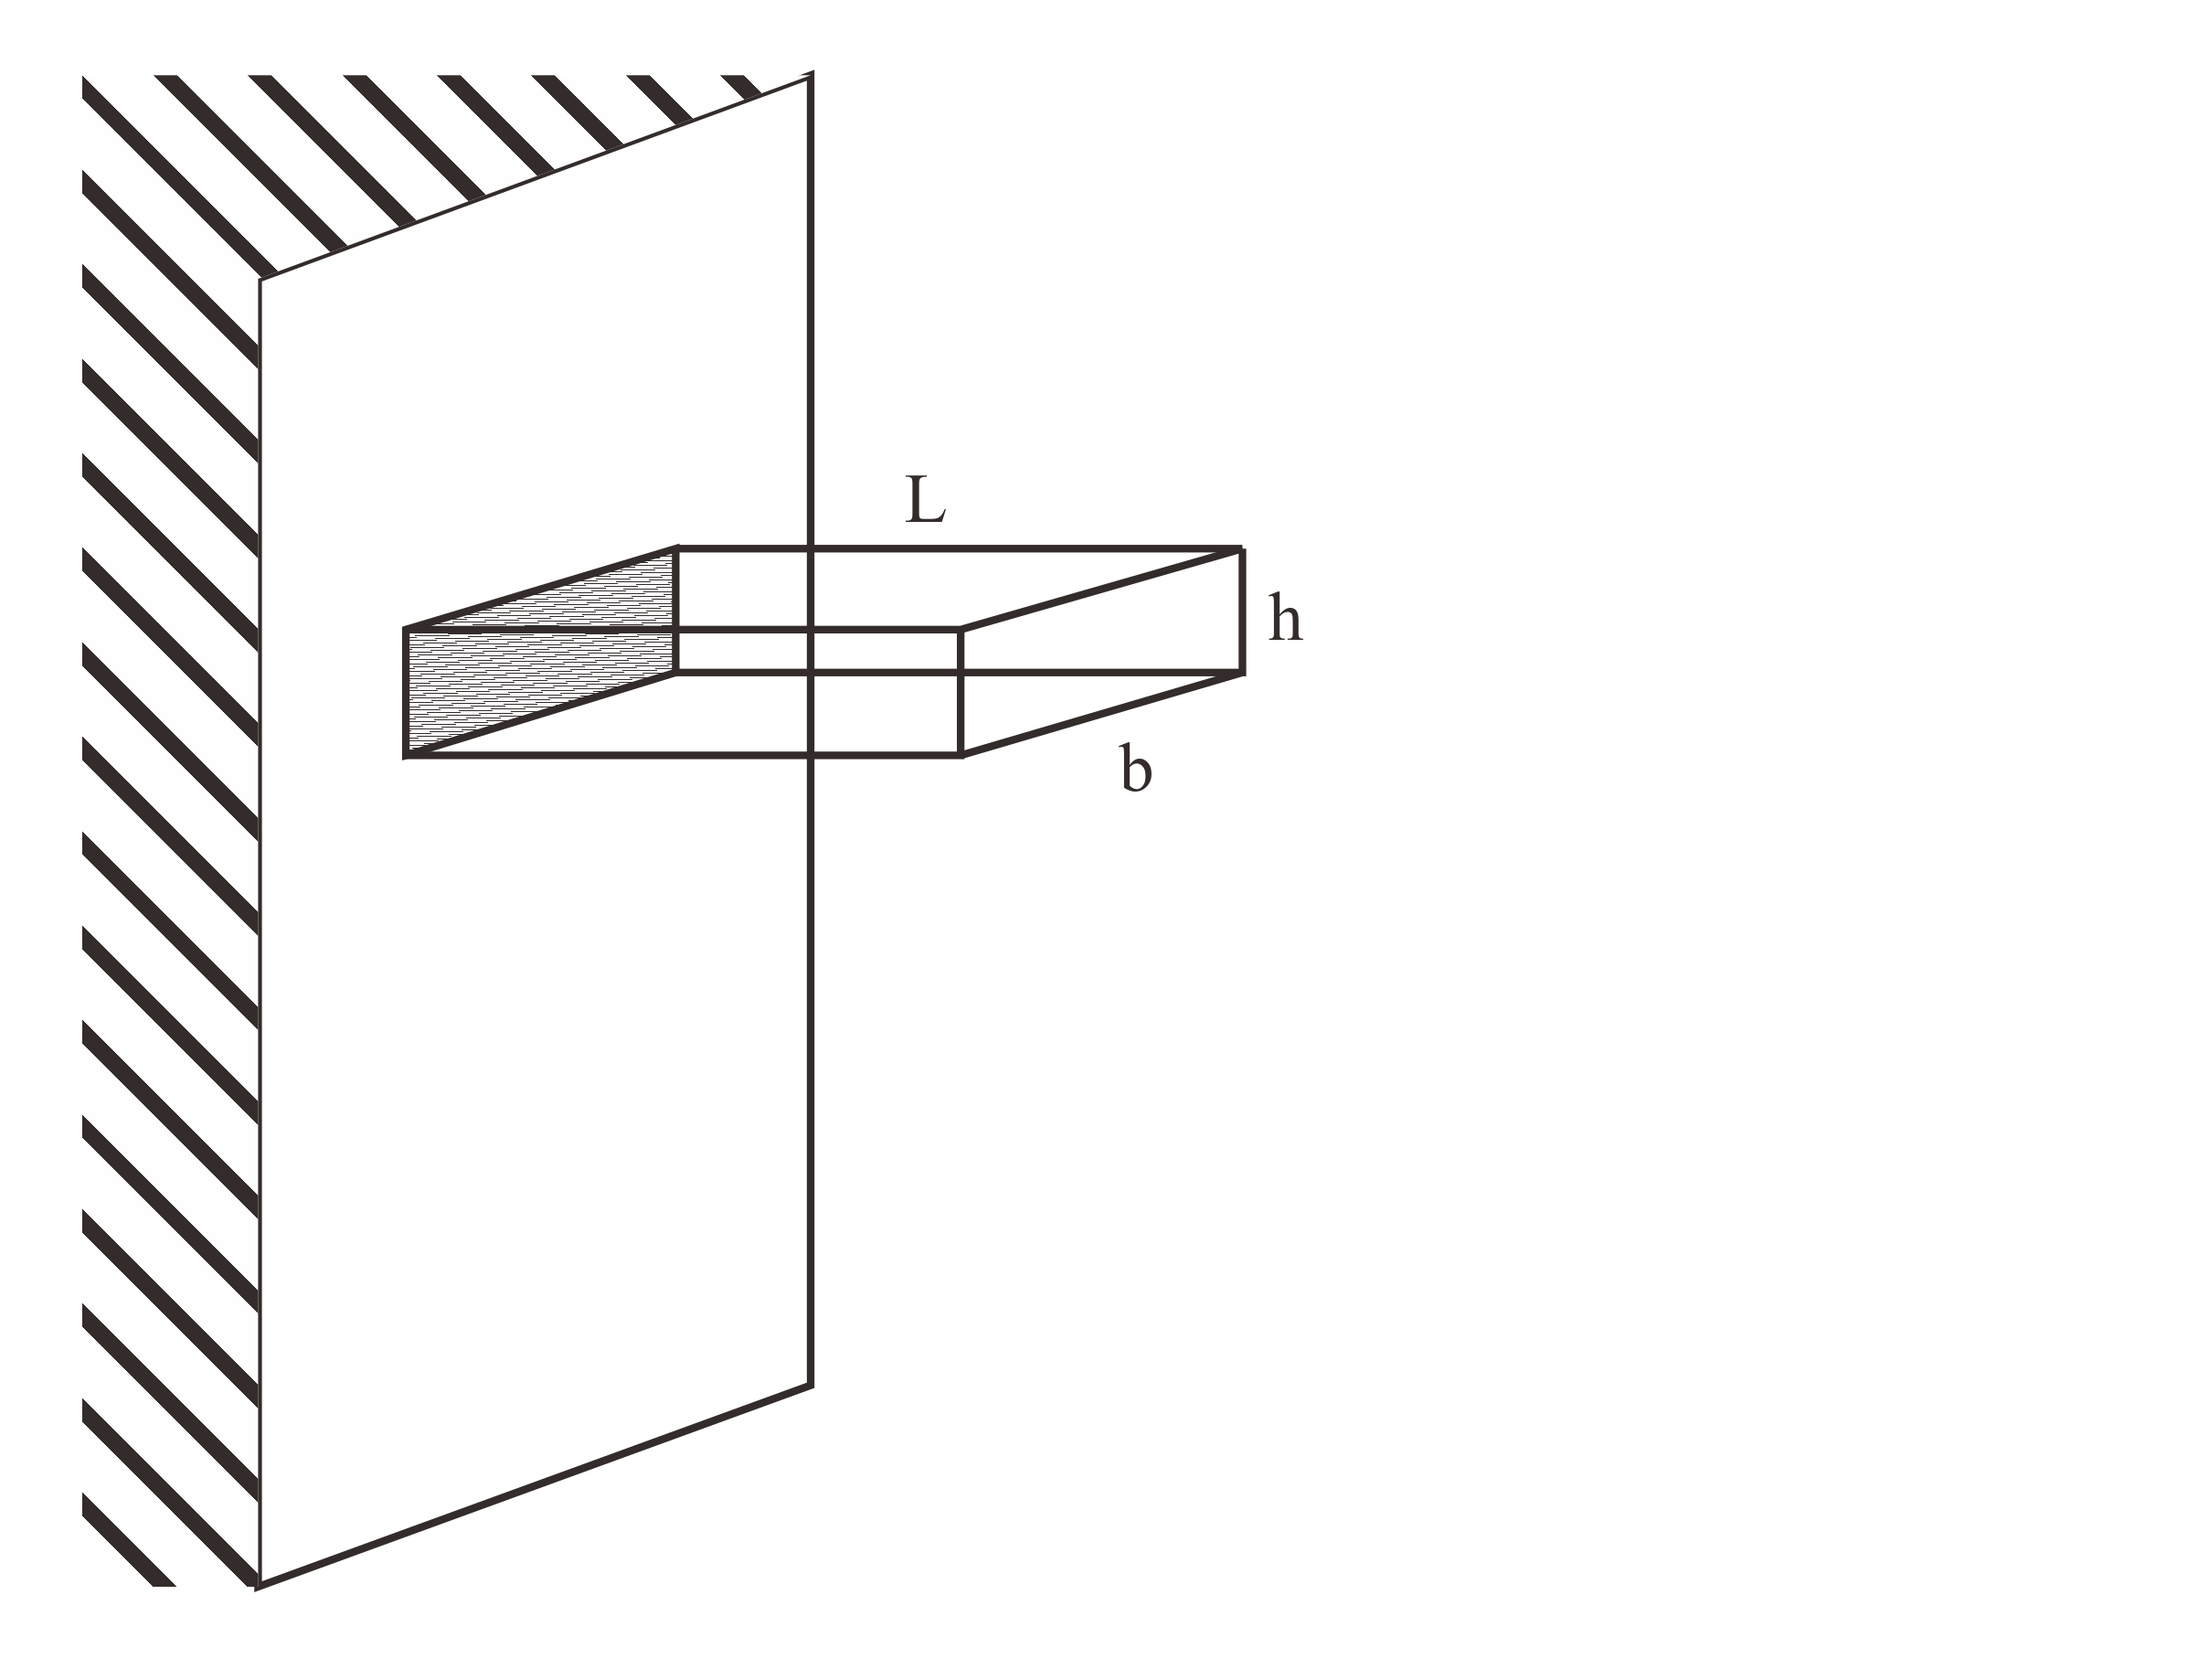
\includegraphics[width=0.5\linewidth]{picture/3dmodellinearelasticity}
	\caption{3D Model of cantilever beam. We use gravity force as the body force \textbf{f} and fixed the left part of the beam, and then we give a 1 Newton weight force act on the right part of the beam as the neumann boundary condition \textbf{q}.}
	\label{fig:3dmodel}
\end{figure}
With the help of FreeFem++ software, we created a 2D and 3D model as shown in figure \ref{fig:3dmodel}, then we solve the displacement vector ($u$, $v$). After solving the displacement, we calculate $\sigma$ which stand for stress force acting on surface of the cantilever beam using equation below:
\begin{equation*}
\begin{aligned}[center]
\sigma = (d \lambda^2 + 4\lambda\mu)div(u)^2 + (4\mu^2 |e[u]|^2),\ d=2,3\\
\lambda\ \text{(Lame's first parameter)}\ := \frac{E\nu}{(1+\nu)(1-2\nu)}\\
\mu\ \text{Lame's second parameter}\ := \frac{E}{2(1+\nu)}
\end{aligned}
\end{equation*}
\newpage
\section{Result and Discussion}
We solved the problem in \eqref{eq:weaklinear} by using P1 finite element method on FreeFEM++, where $u$ and $v$ calculated for division number of mesh = 32. In the figure \ref{fig:displacementresult} we can see the deformation of the cantilever beam in 2D and 3D graphics.
\begin{figure}[h!]
	\begin{subfigure}[b]{0.5\linewidth}
		\centering
		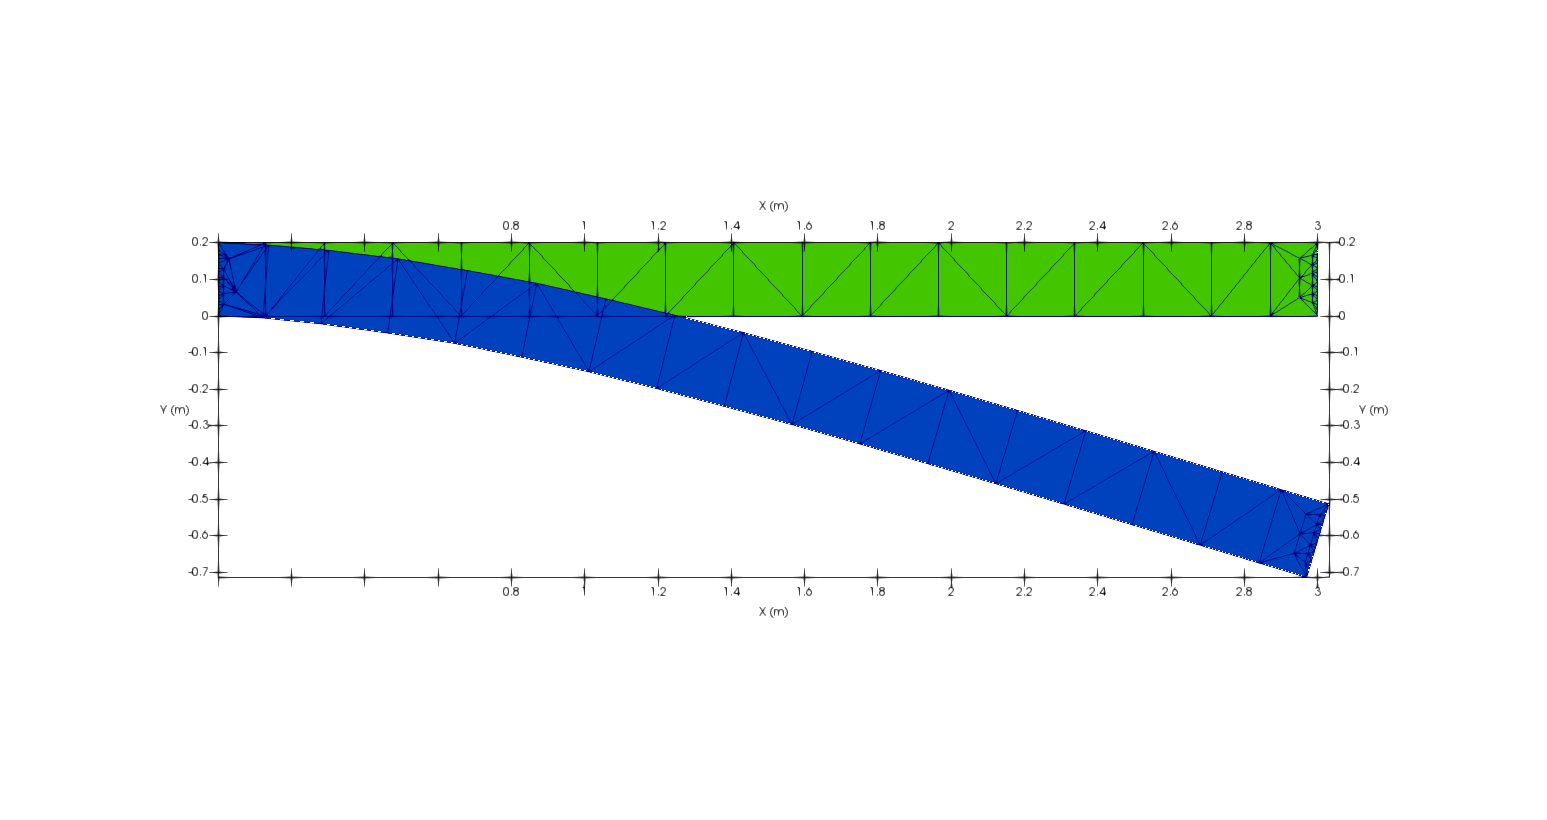
\includegraphics[width=\linewidth]{picture/conference/2d1}
		\caption{Deformation in 2D. Green line show condition before gravity and weight force applied to the domain. Red line show condition after we solve linear elasticity with gravity and weight force applied to the domain. Maximal Displacement ($u = 0.03\ [m]$)}
		\label{fig:2dresult}
	\end{subfigure}
\quad
	\begin{subfigure}[b]{0.5\linewidth}
		\centering
		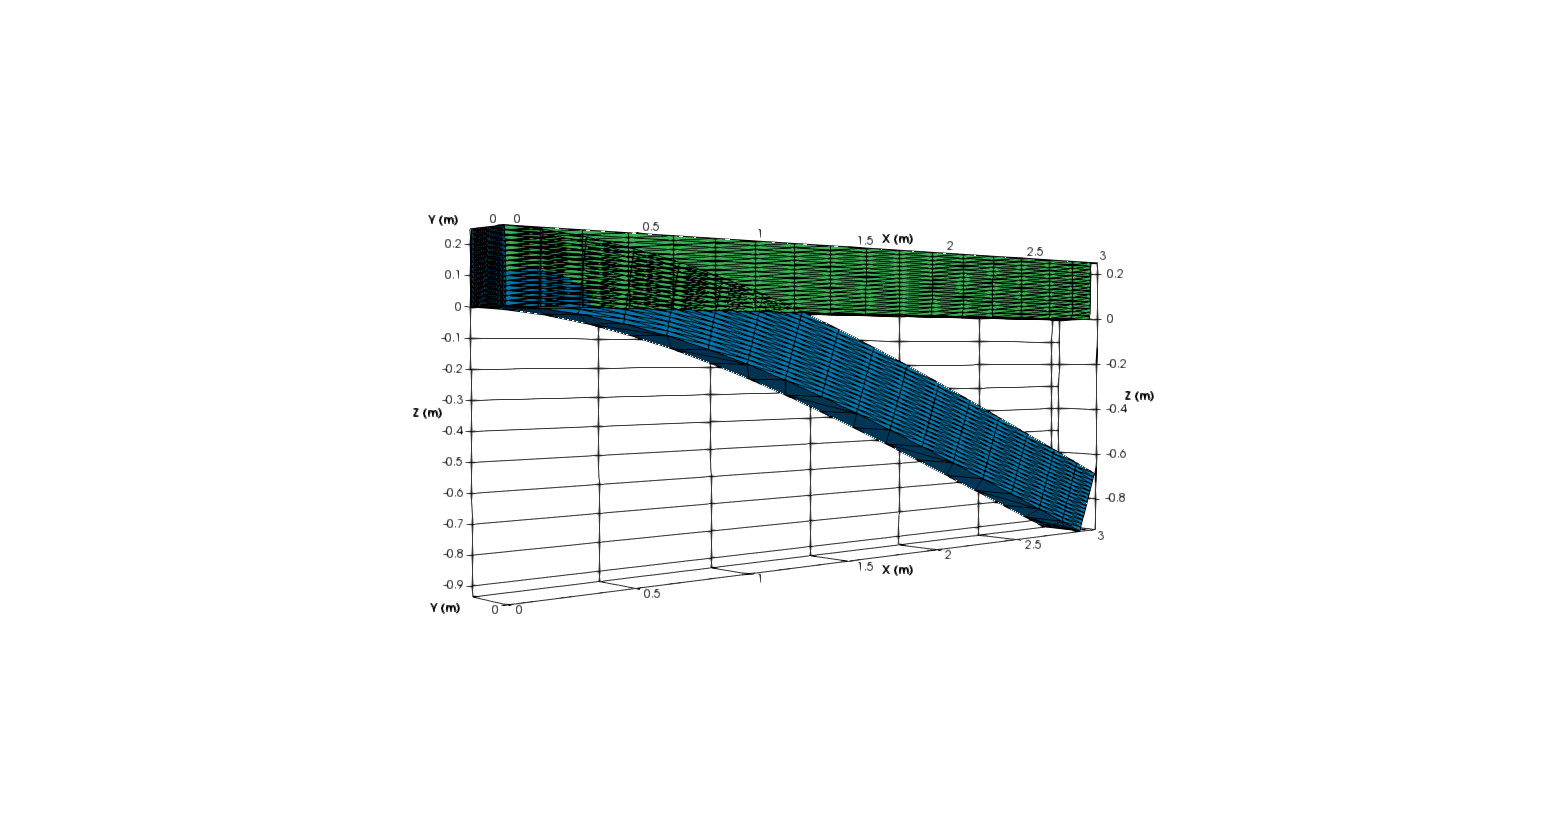
\includegraphics[width=\linewidth]{picture/conference/3d1}
		\caption{Deformation in 3D. Green line show condition before gravity and weight force applied to the domain. Red line show condition after we solve linear elasticity with gravity and weight force applied to the domain. Maximal Displacement ($u = 0.05\ [m]$)}
		\label{fig:3dresult}
	\end{subfigure}
\caption{Deformation in 2D and 3D}
\label{fig:displacementresult}
\end{figure}
\newline
While in the figure \ref{fig:stresstensor} we can see result from calculating the stress tensor on 2D and 3D case.
\begin{figure}[h!]
	\begin{subfigure}[b]{0.5\linewidth}
		\centering
		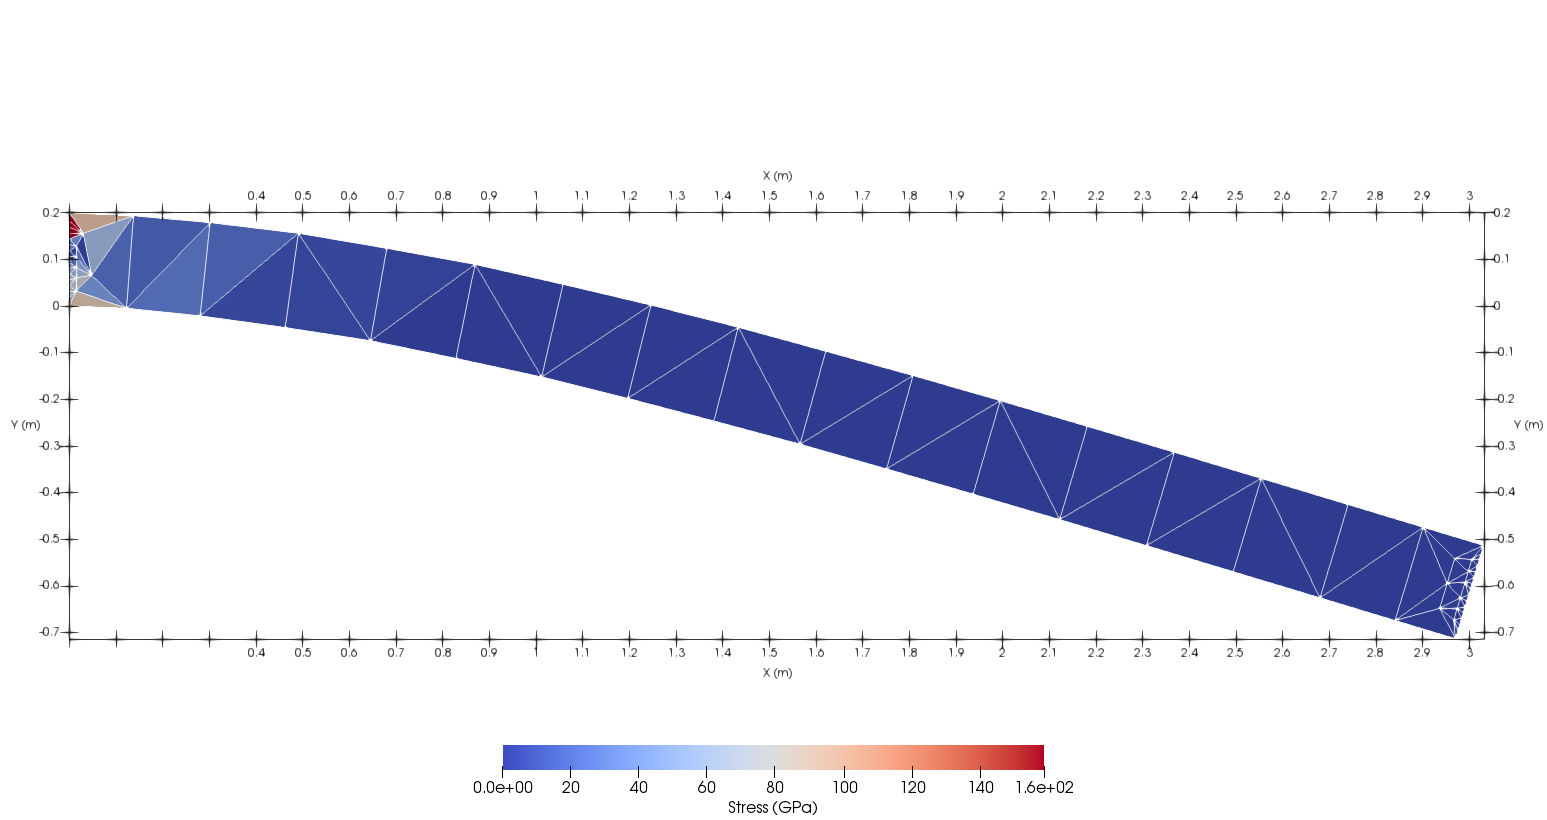
\includegraphics[width=\linewidth]{picture/conference/2dstress}
		\caption{Calculated $\sigma$ on 2D case. The value of $\sigma$ on the domain, maped by the color in the picture with respect to the color palette on the lower side of the graph. Maximal stress given on the surface ($\sigma = 158.612\ [GPa]$)}
		\label{fig:2dstress}
	\end{subfigure}
\quad
	\begin{subfigure}[b]{0.5\linewidth}
		\centering
		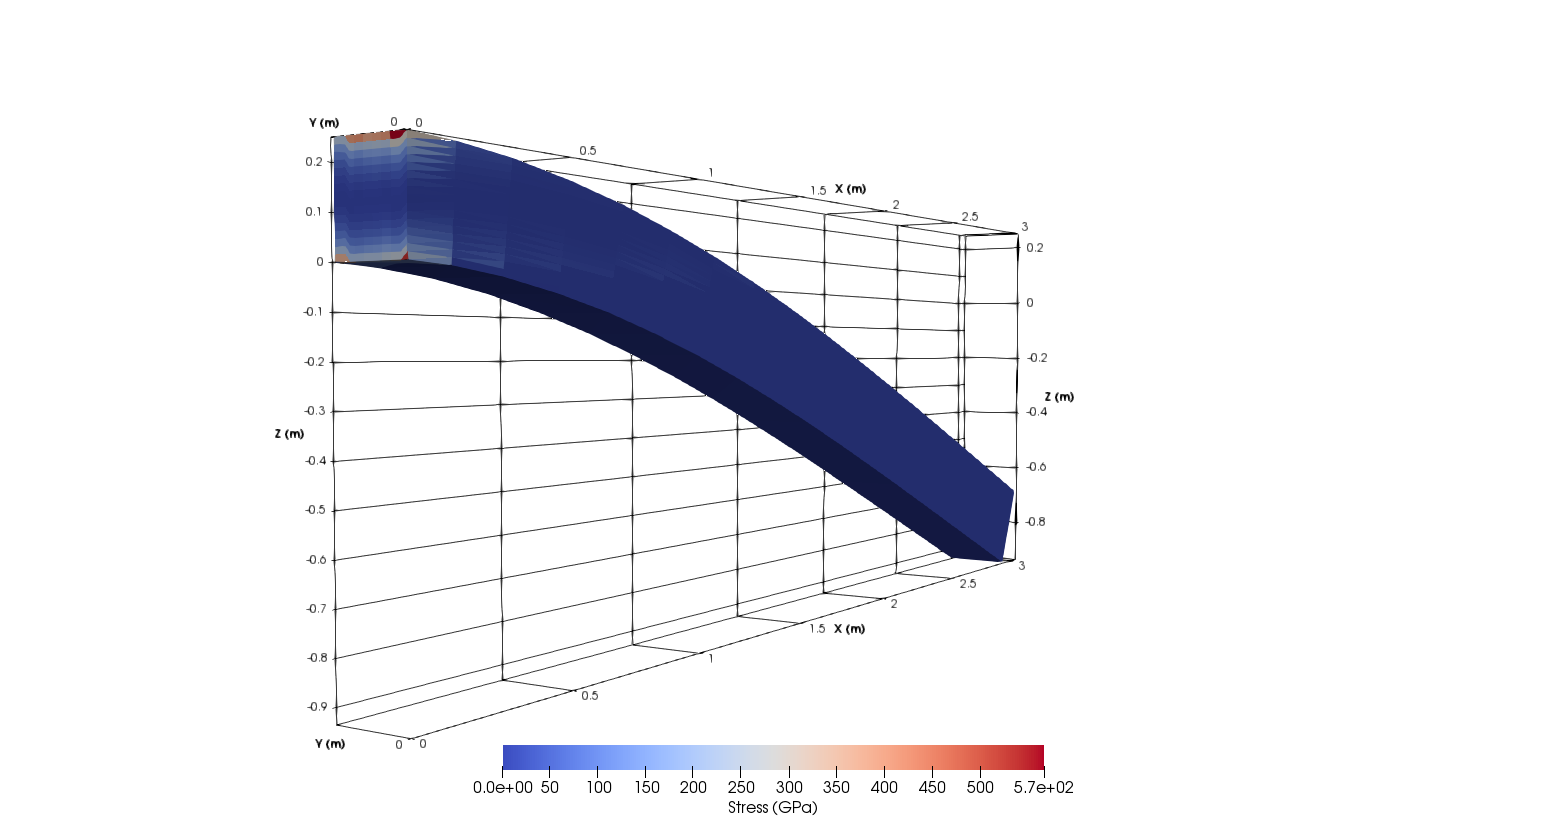
\includegraphics[width=\linewidth]{picture/conference/3dstress}
		\caption{Calculated $\sigma$ on 3D case. The value of $\sigma$ on the domain, maped by the color in the picture with respect to the color palette on the lower side of the graph. Maximal stress given on the surface ($\sigma = 567.034\ [GPa]$)}
		\label{fig:3dstress}
	\end{subfigure}
\caption{Stress Tensor in 2D and 3D}
\label{fig:stresstensor}
\end{figure}
\newpage
On the figure \ref{fig:comparison}, we can see comparison of calculated surface stress on 2D and 3D case (sliced on the side).
\begin{figure}[h!]
	\begin{subfigure}[b]{0.5\linewidth}
		\centering
		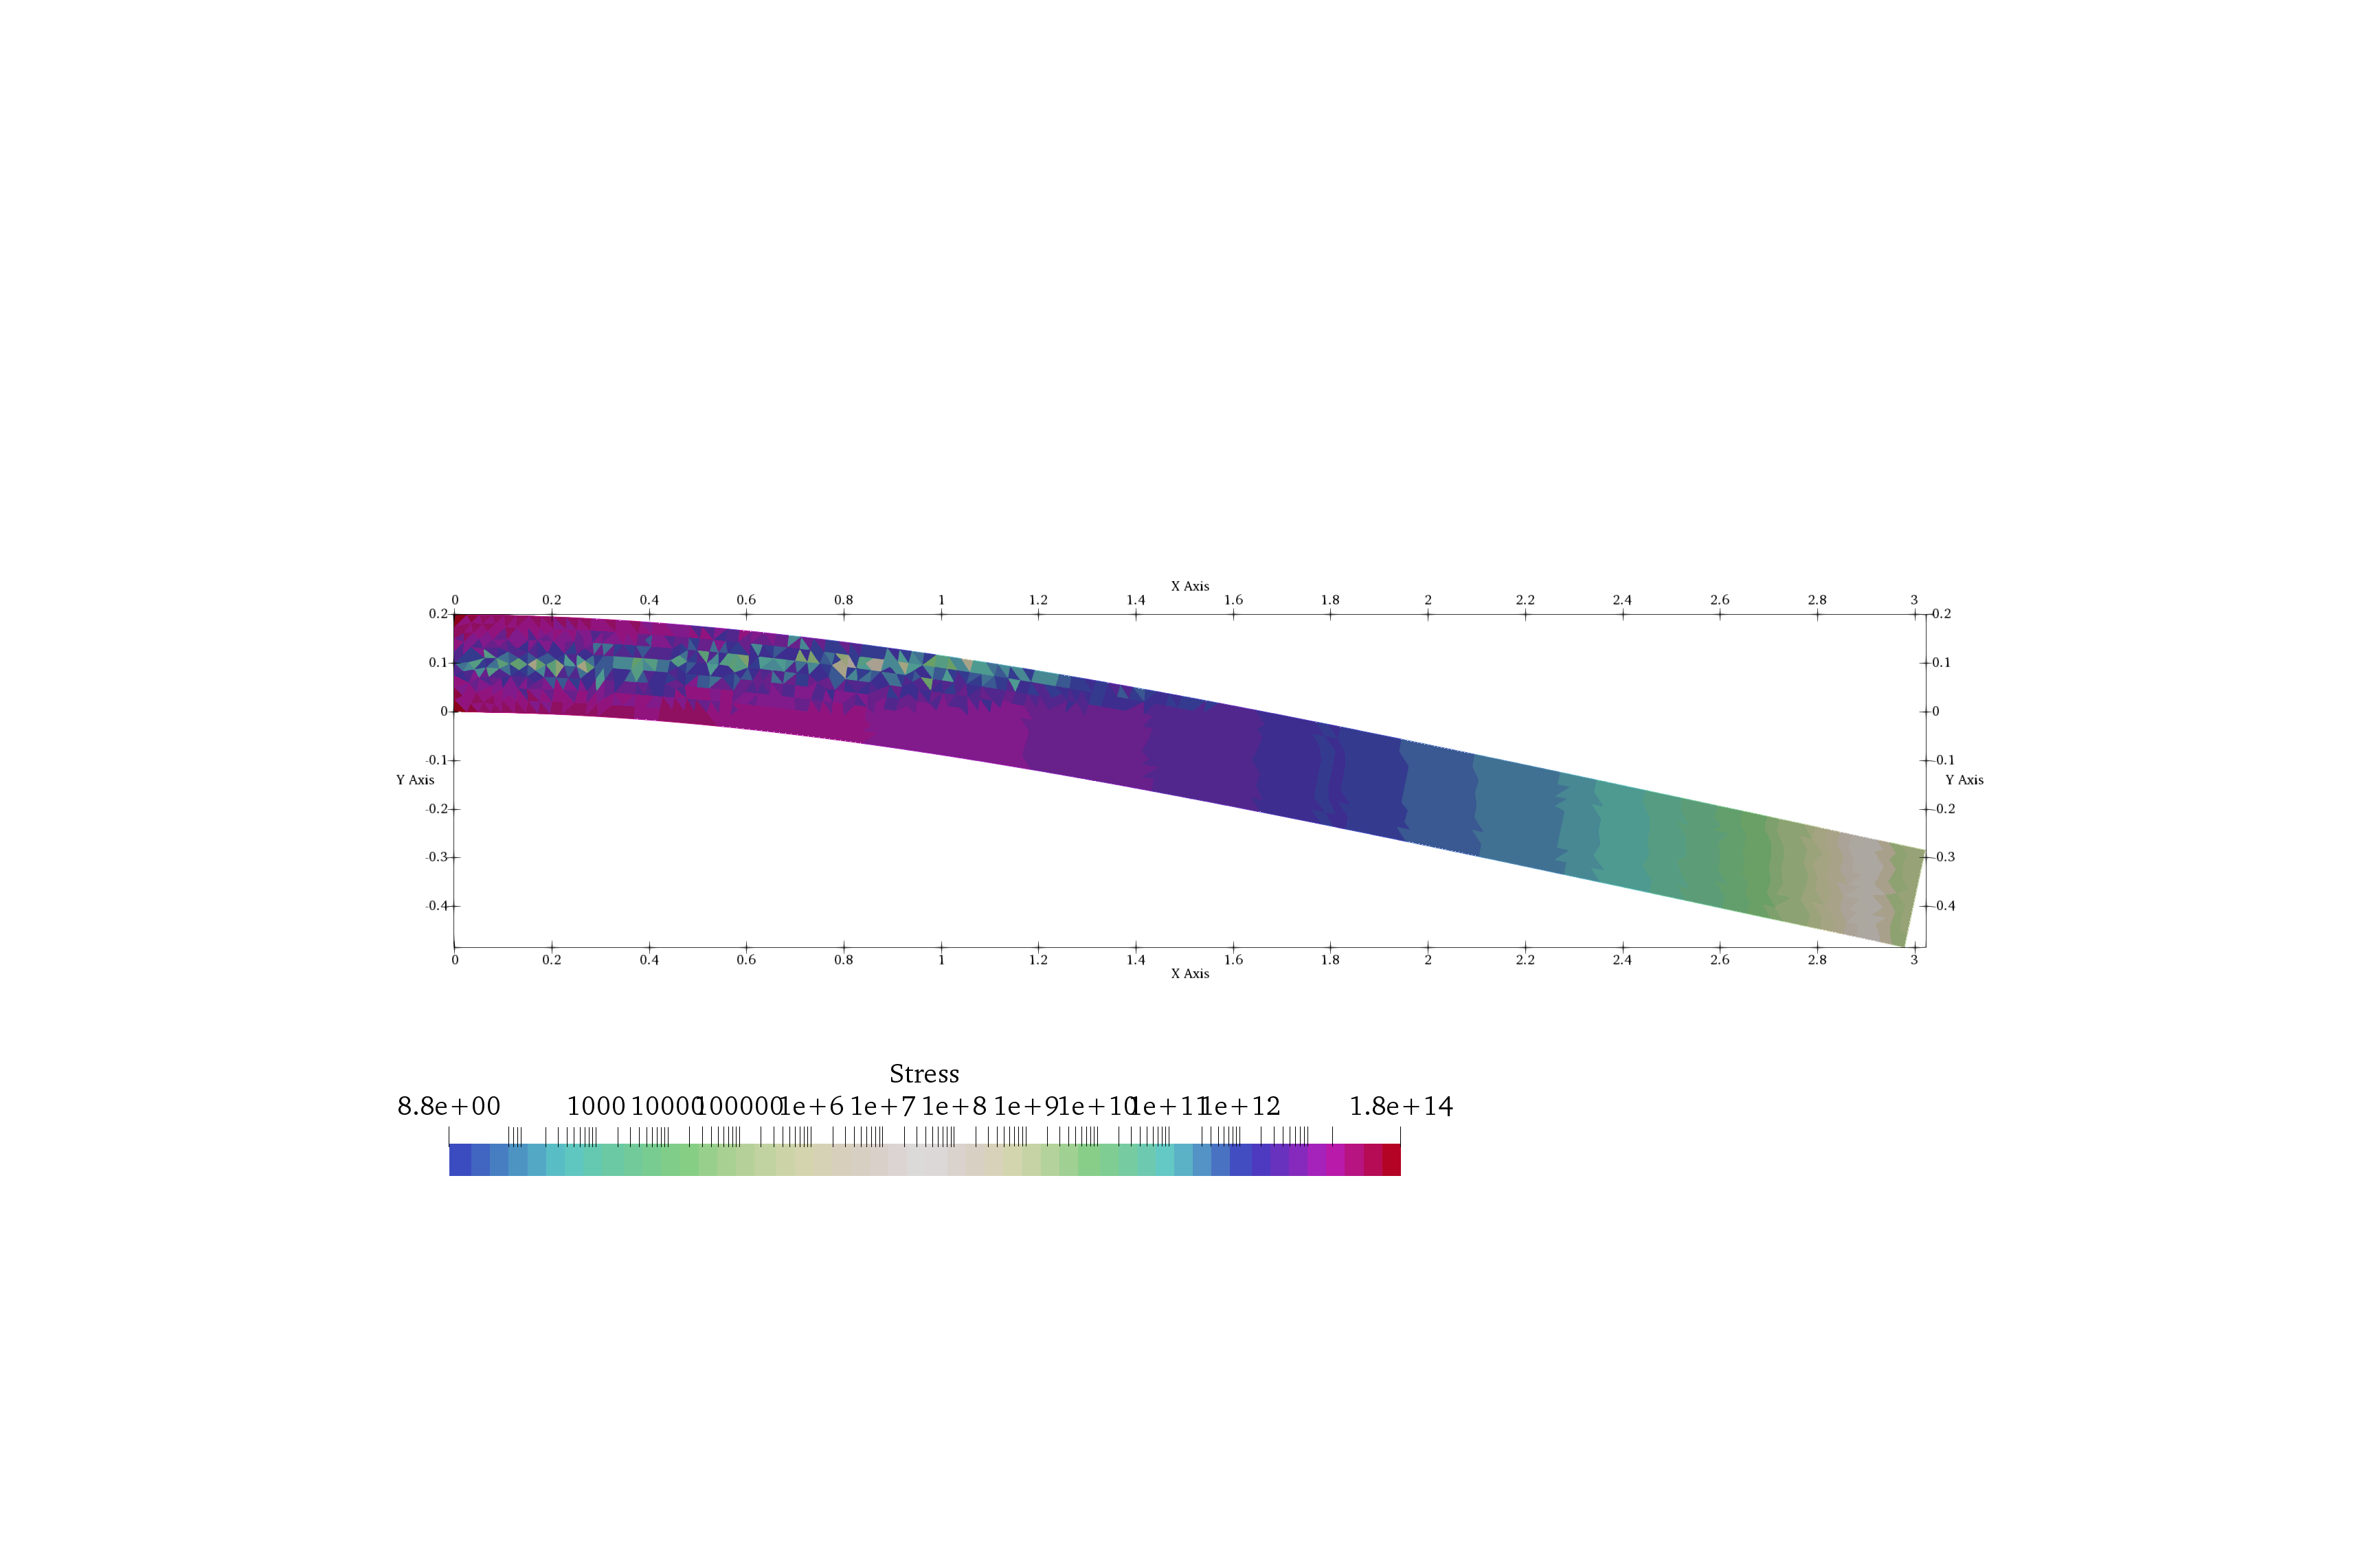
\includegraphics[width=\linewidth]{picture/conference/2dstress1}
		\caption{Calculated surface stress on 2D}
	\end{subfigure}
	\quad
	\begin{subfigure}[b]{0.5\linewidth}
		\centering
		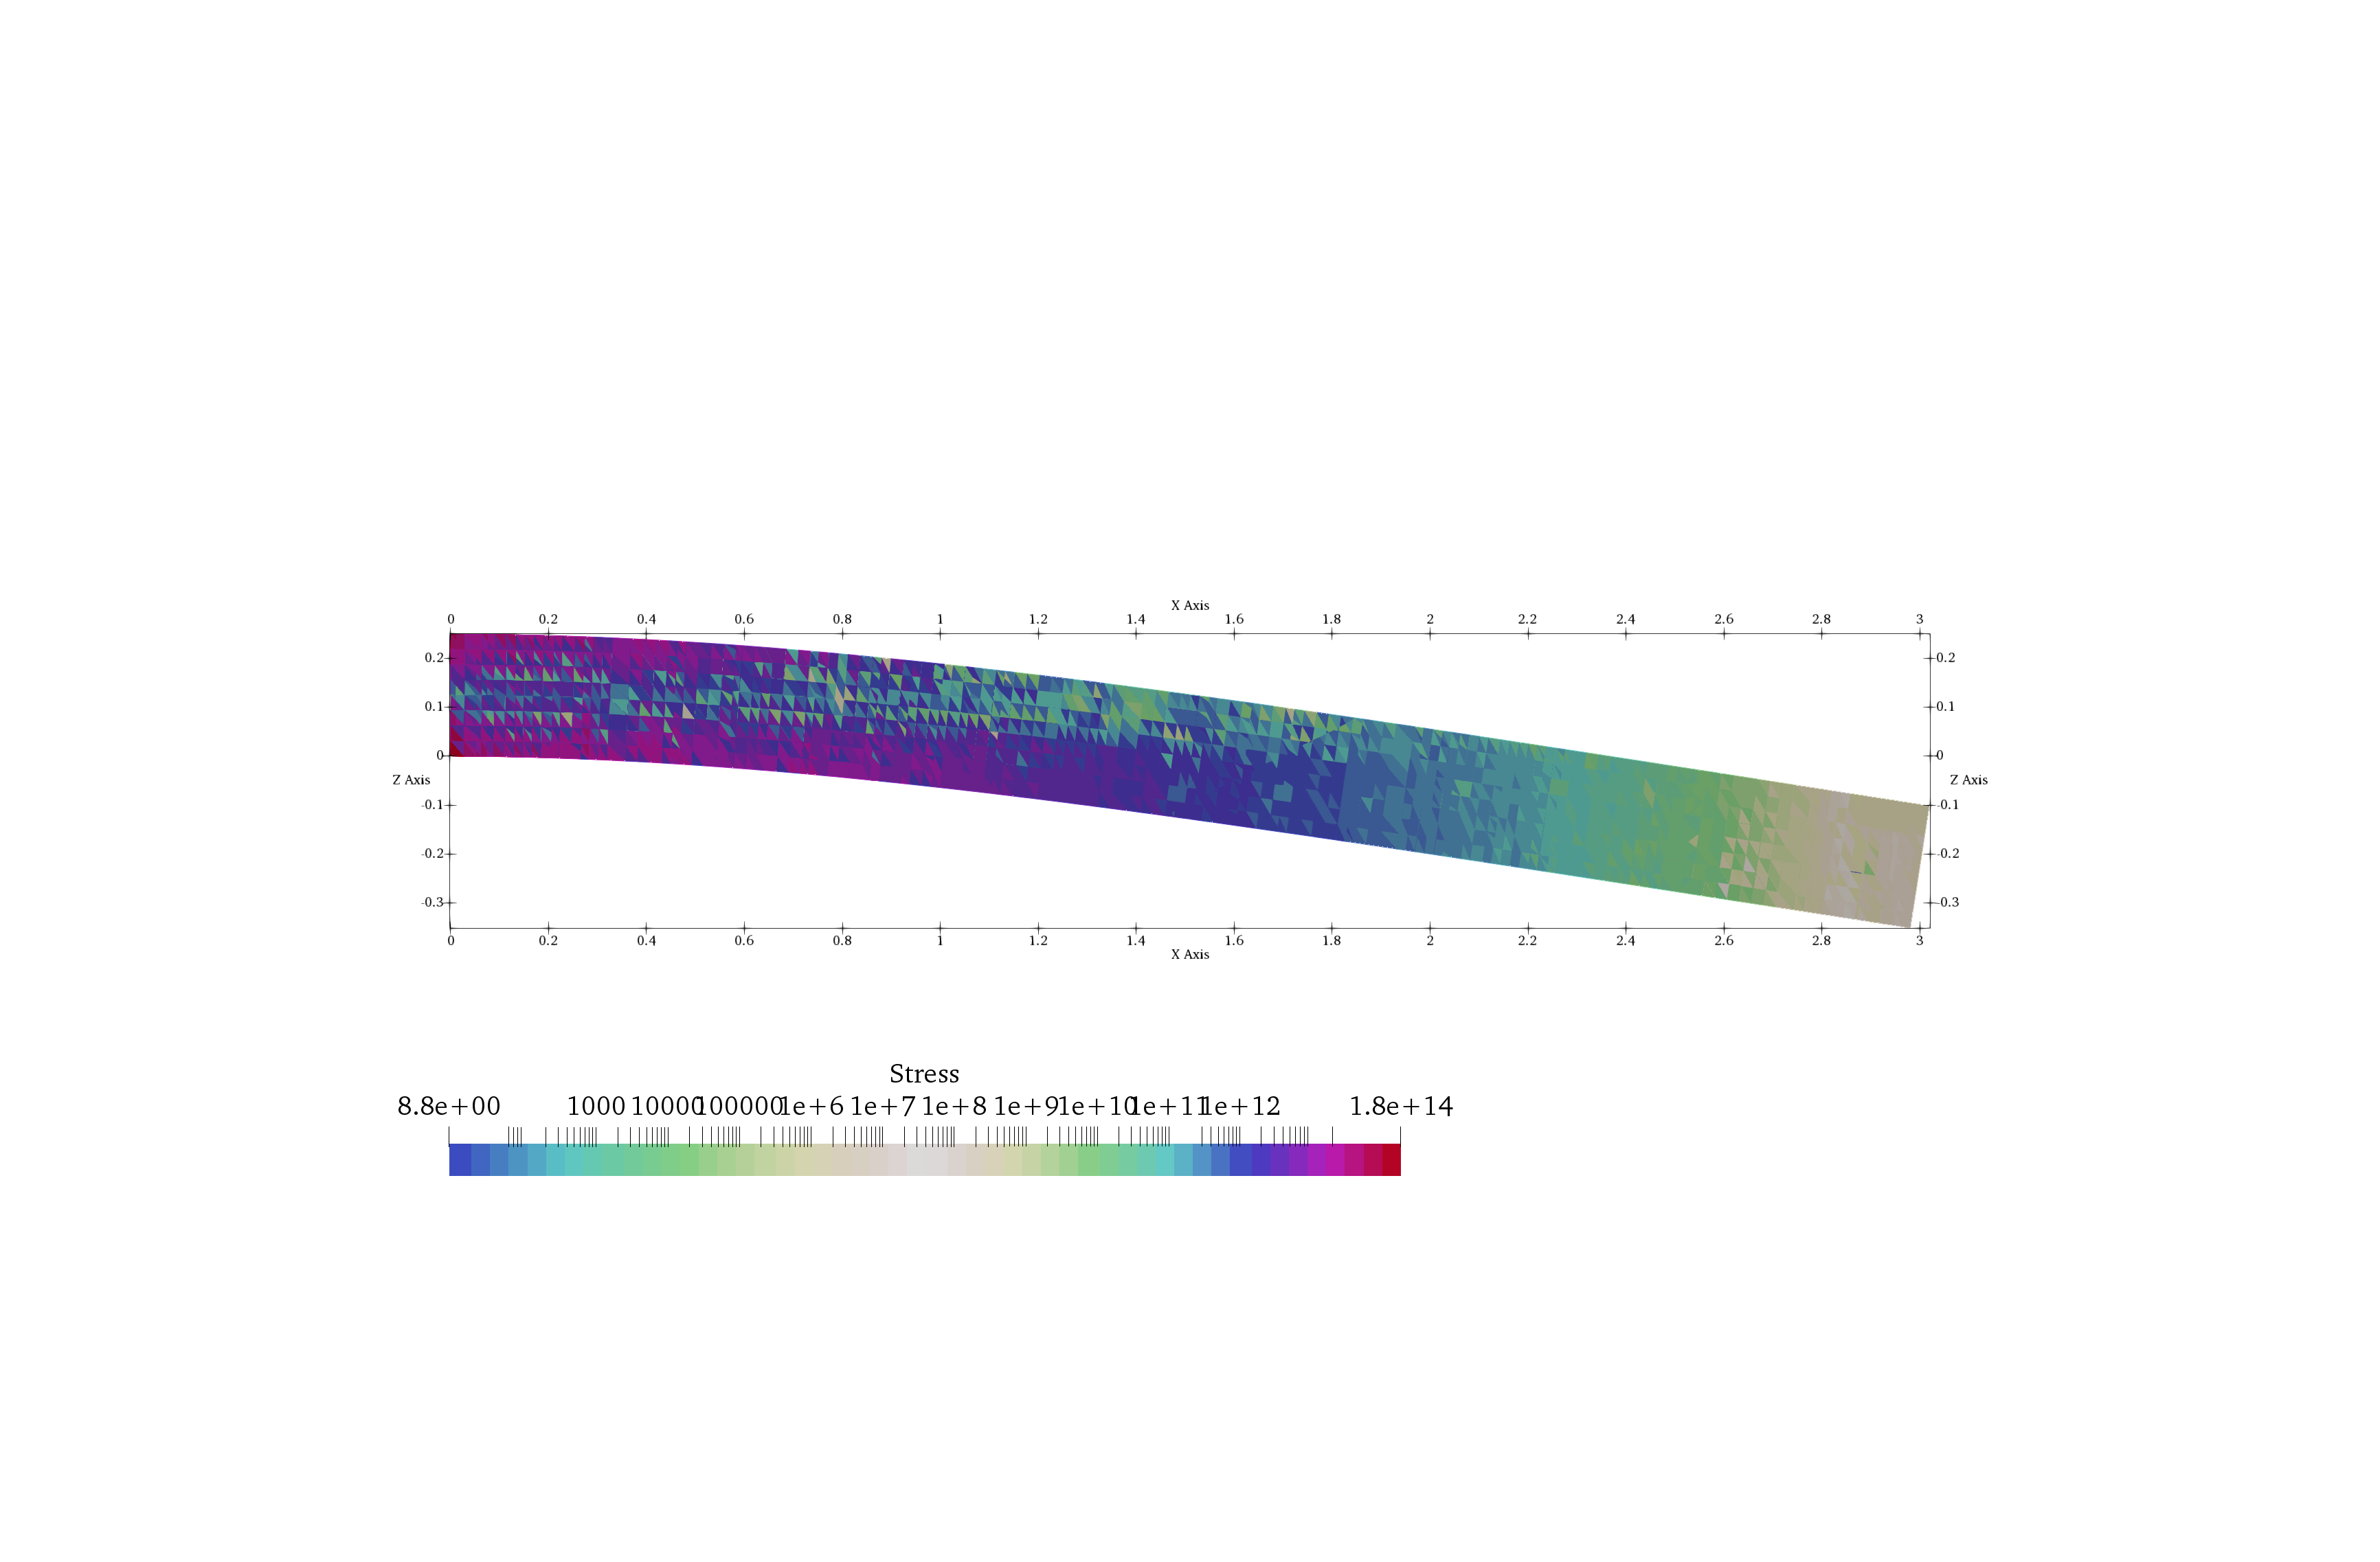
\includegraphics[width=\linewidth]{picture/conference/3dstress1}
		\caption{Calculated surface stress on 3D}
		\label{}
	\end{subfigure}
	\caption{Comparison of Stress Tensor in 2D and 3D}
	\label{fig:comparison}
\end{figure}
\newline
On the figure \ref{fig:3dsliceview} below, we can see the result from sliced view on 3D case, in this case, we sliced through the Y-normal plane of the 3D model.
\begin{figure}[h!]
	\begin{subfigure}[b]{0.5\linewidth}
		\centering
		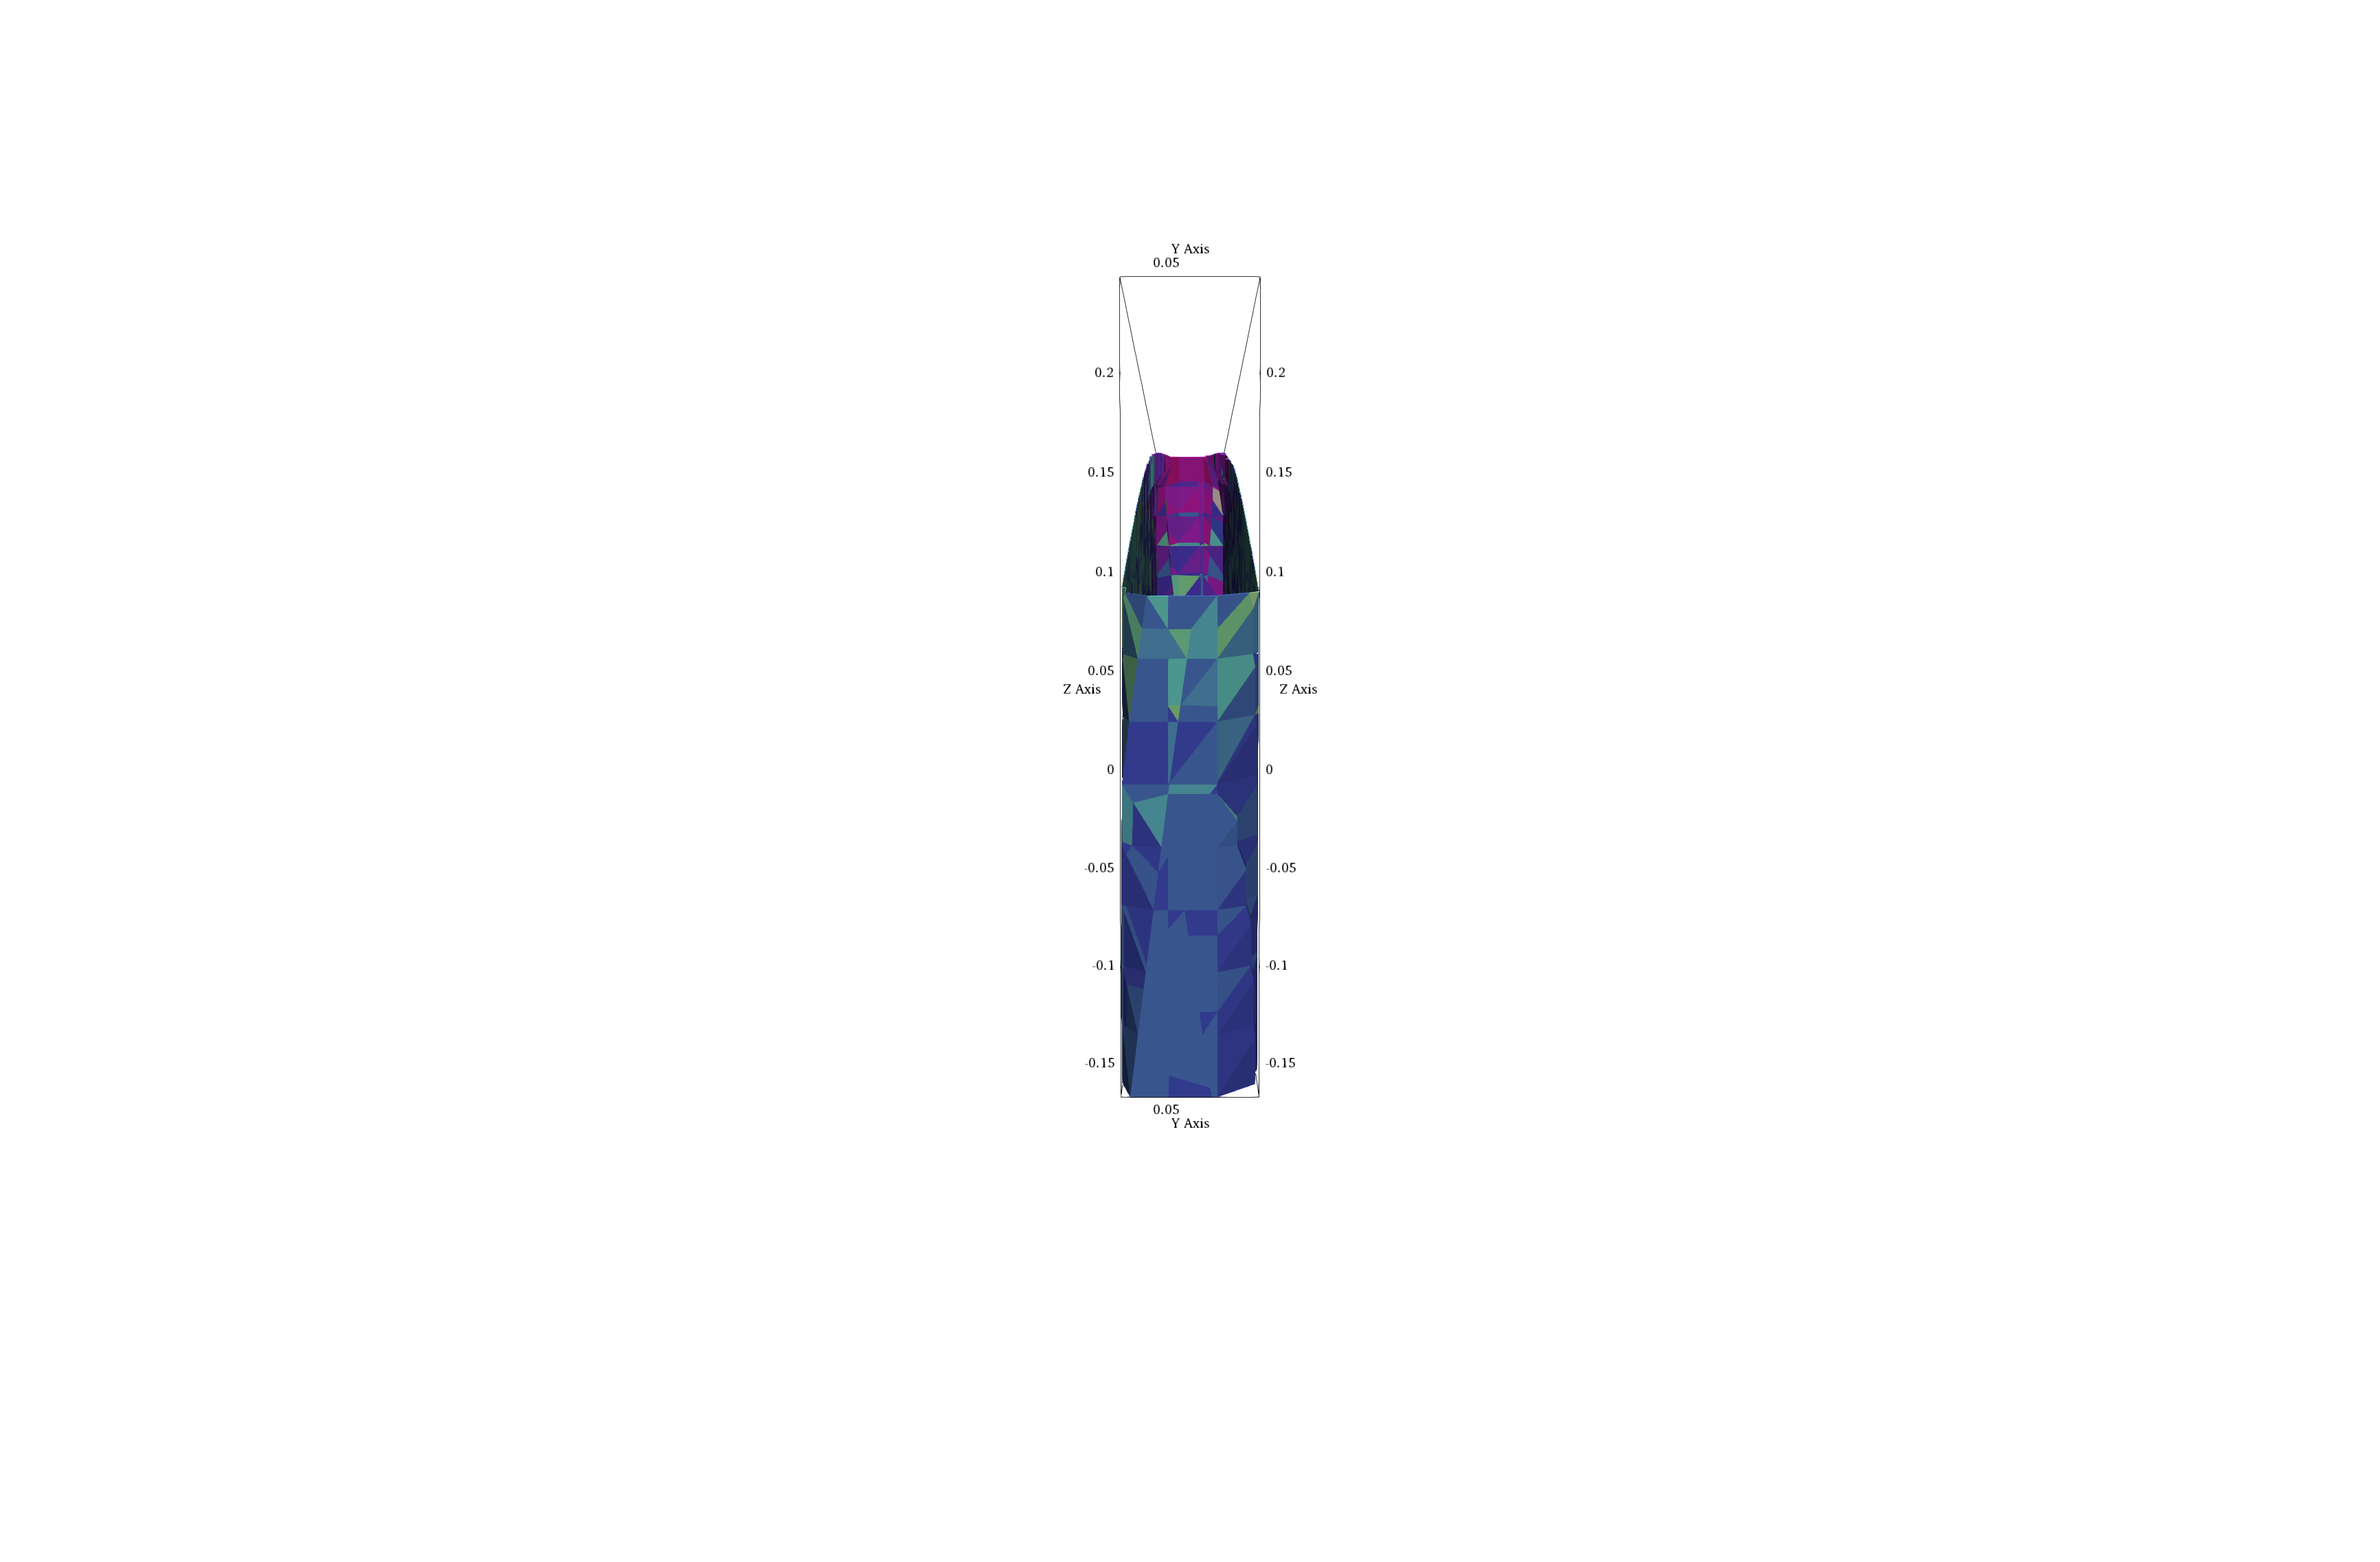
\includegraphics[width=\linewidth]{picture/conference/3dslice4}
		\caption{Front View}
	\end{subfigure}
	\quad
	\begin{subfigure}[b]{0.5\linewidth}
		\centering
		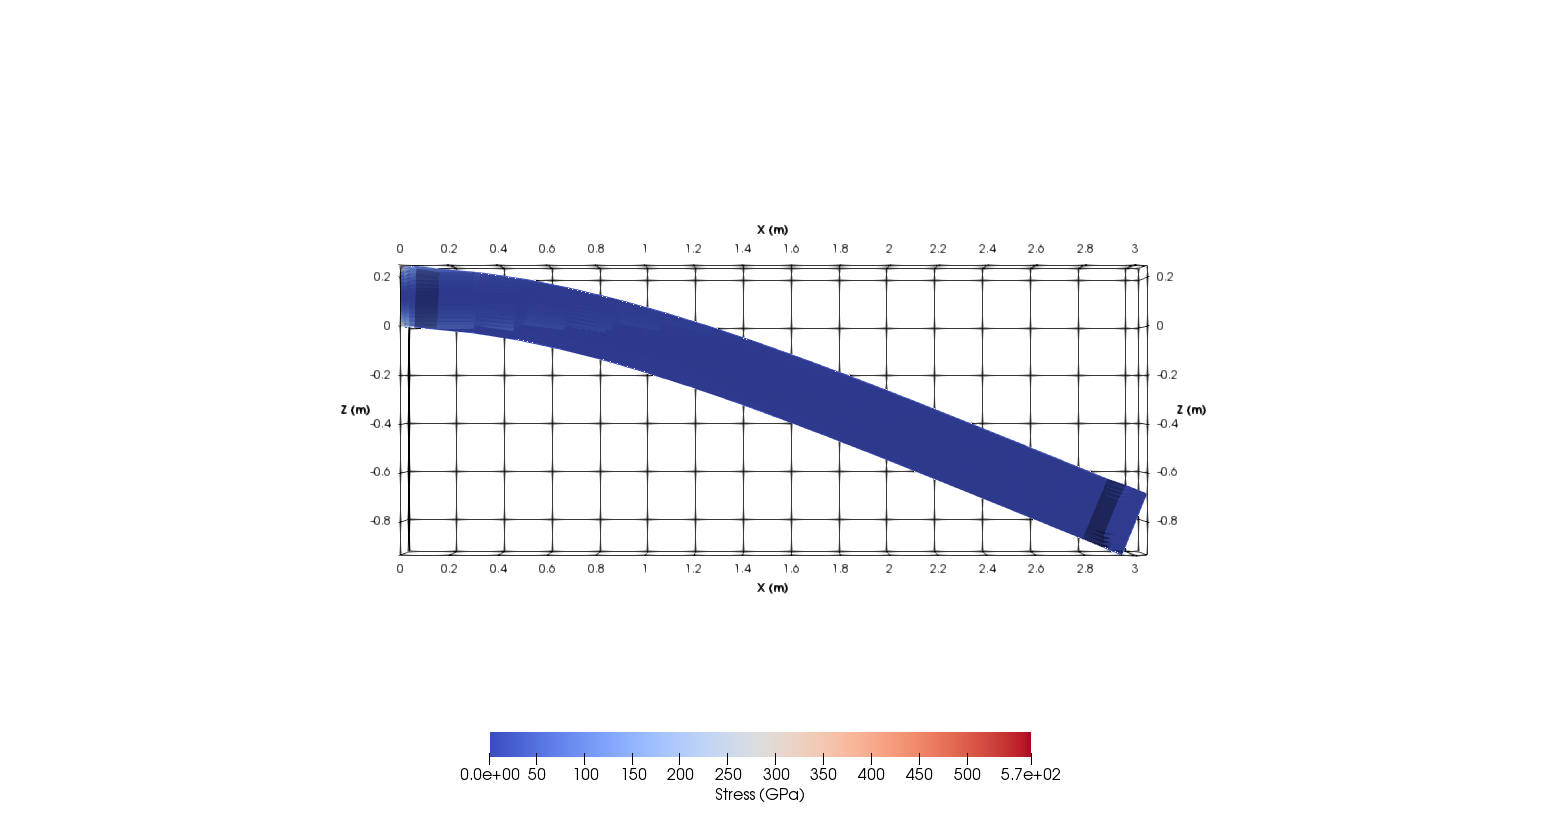
\includegraphics[width=\linewidth]{picture/conference/3dslice6}
		\caption{Right View}
	\end{subfigure}
	\quad
	\begin{subfigure}[b]{0.5\linewidth}
		\centering
		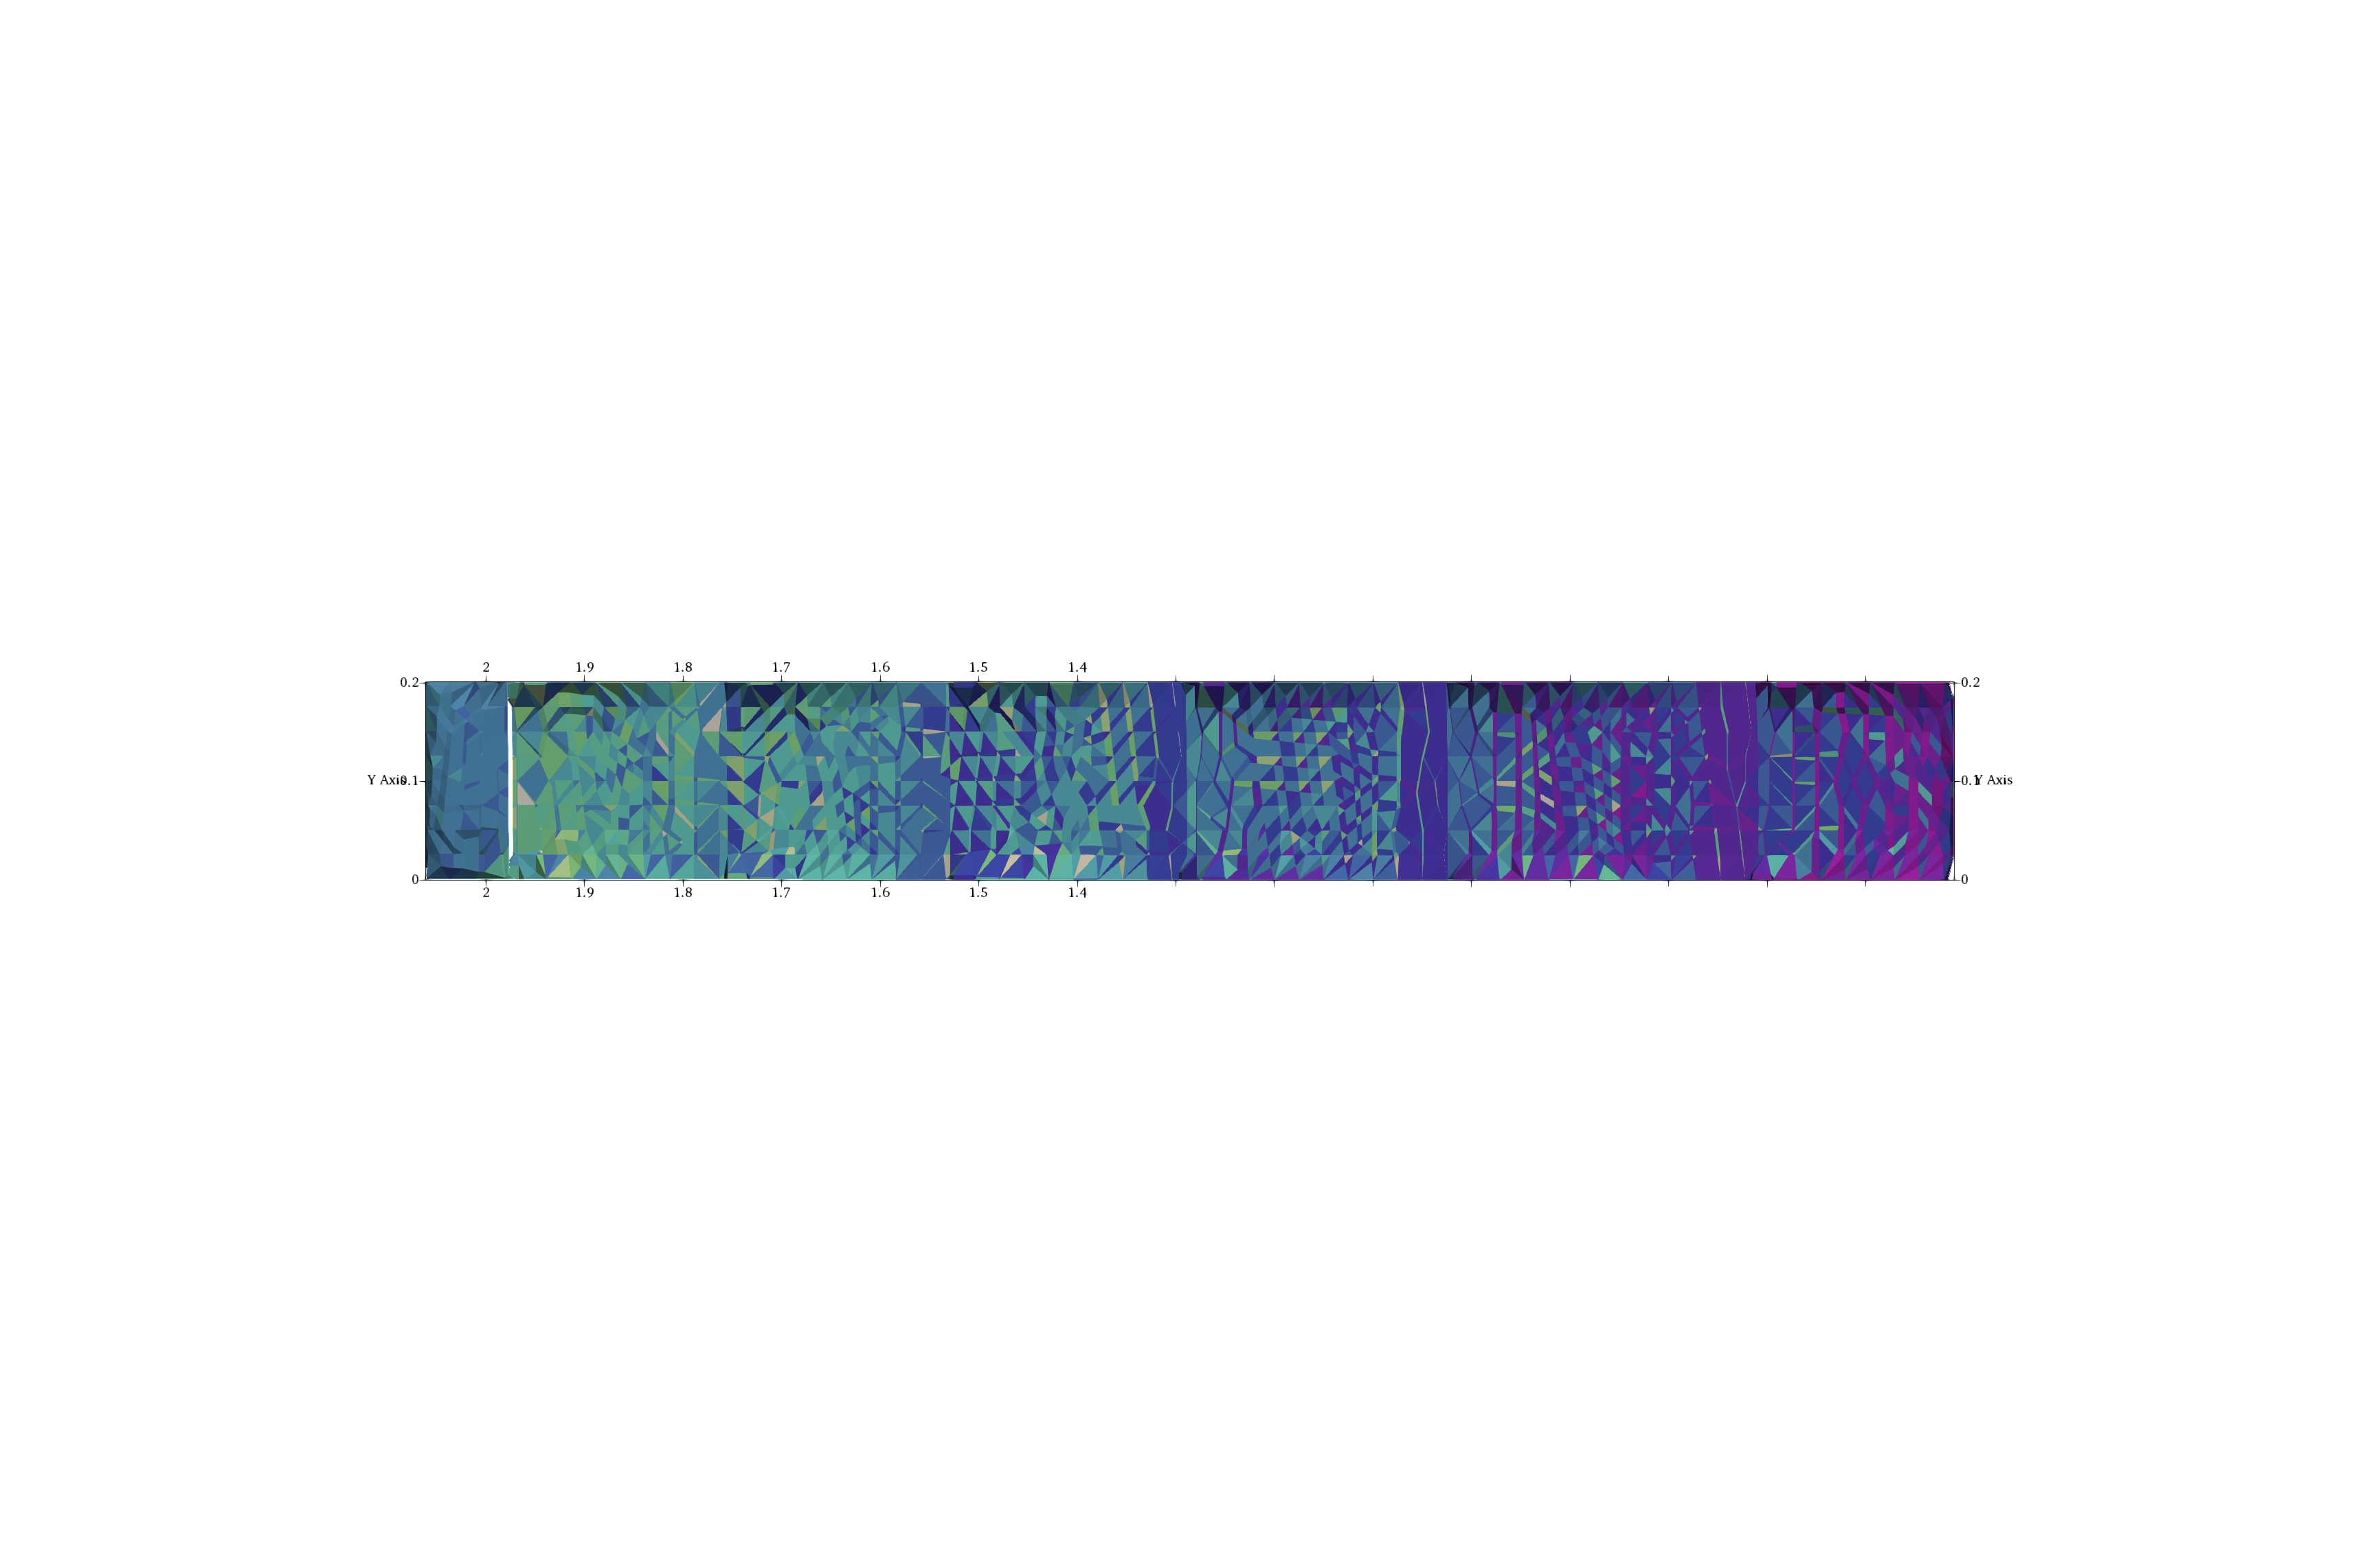
\includegraphics[width=\linewidth]{picture/conference/3dslice8}
		\caption{Top View}
	\end{subfigure}
	\quad
	\begin{subfigure}[b]{0.5\linewidth}
		\centering
		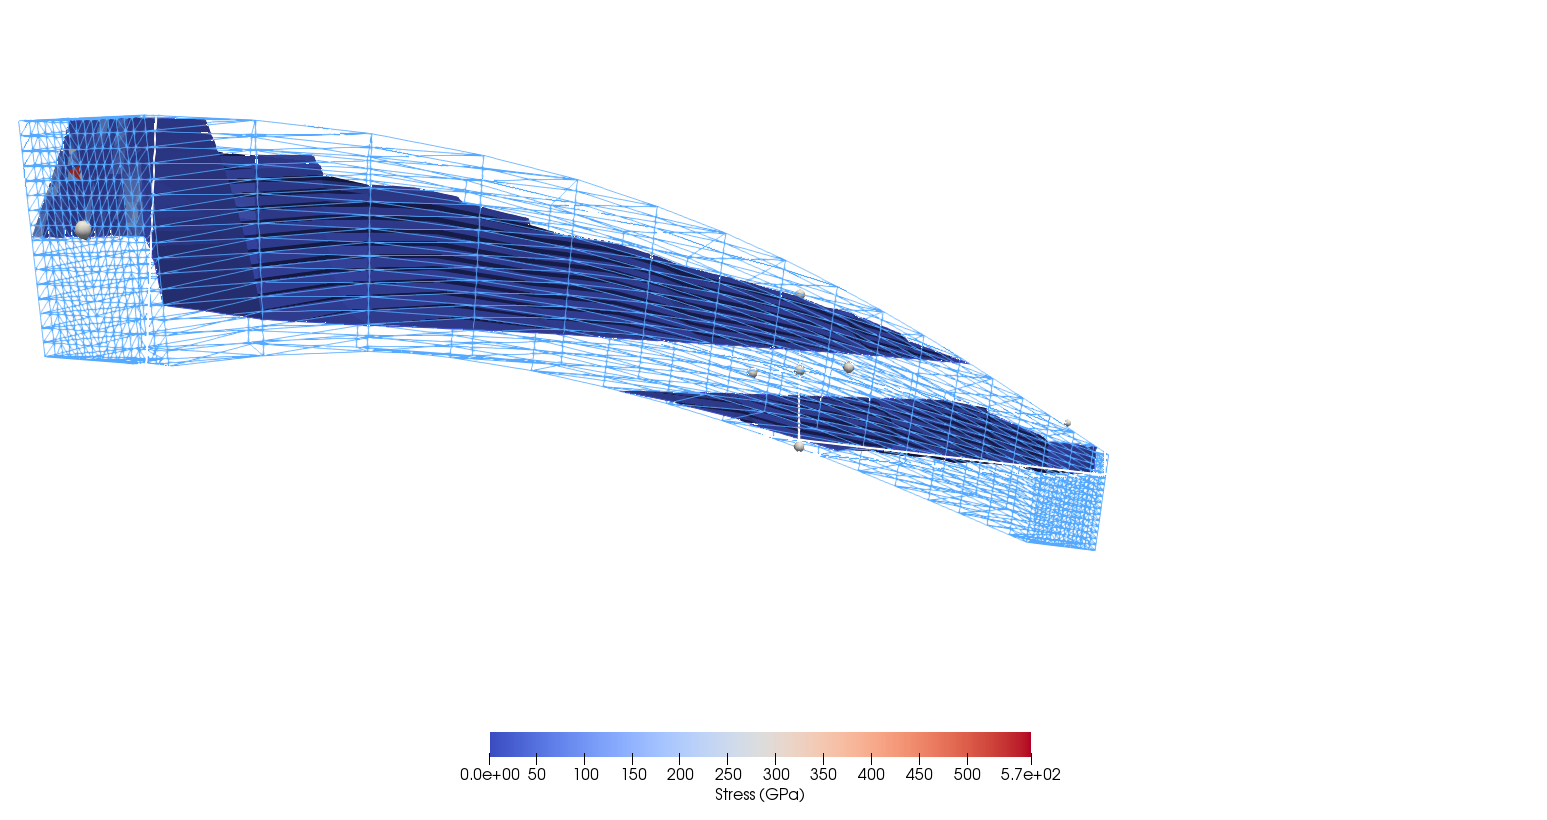
\includegraphics[width=\linewidth]{picture/conference/3dslice9}
		\caption{Wireframed-Sliced View}
	\end{subfigure}
	\caption{3D Sliced View}
	\label{fig:3dsliceview}
\end{figure}
\newpage
\subsection{Convergence Analysis}
Since we don't have an exact solution for problem \eqref{eq:stronglinear}, we will define $$u_h:= u^k \iff \max|u^k-u^{k-1}| \leq \epsilon$$ $k$ is index of the current solution and $\epsilon$ is a small number, $\epsilon > 0$.\\
There are three types of error that we will compute, Infinity Error, $H^1(\Omega)$ and $L^2(\Omega)$, each of them defined by:
\begin{eqnarray}
||u_h - u||_\infty = \max|u_h-u|\\
||u||^2_{H^1(\Omega)} = \int_\Omega |u|^2 dx + \int_\Omega |\triangledown u|^2 dx\\
||u||^2_{L^2(\Omega)} = \int_\Omega |u|^2 dx
\end{eqnarray}
We can see the result from 2D and 3D case in the figure \ref{fig:errorplot} below:
\begin{figure}[h!]
	\begin{subfigure}[b]{0.5\linewidth}
		\centering
		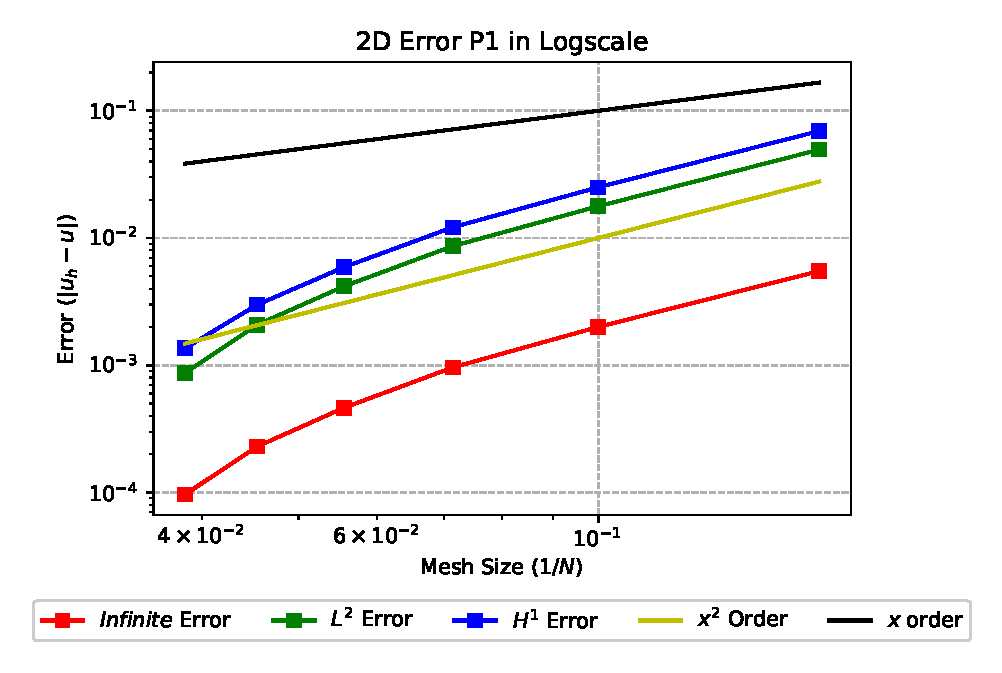
\includegraphics[width=\linewidth]{picture/conference/all2derrorP1}
		\caption{2D Error P1 Plot in Logscale}
		\label{fig:2derrorP1}
	\end{subfigure}
	\quad
	\begin{subfigure}[b]{0.5\linewidth}
		\centering
		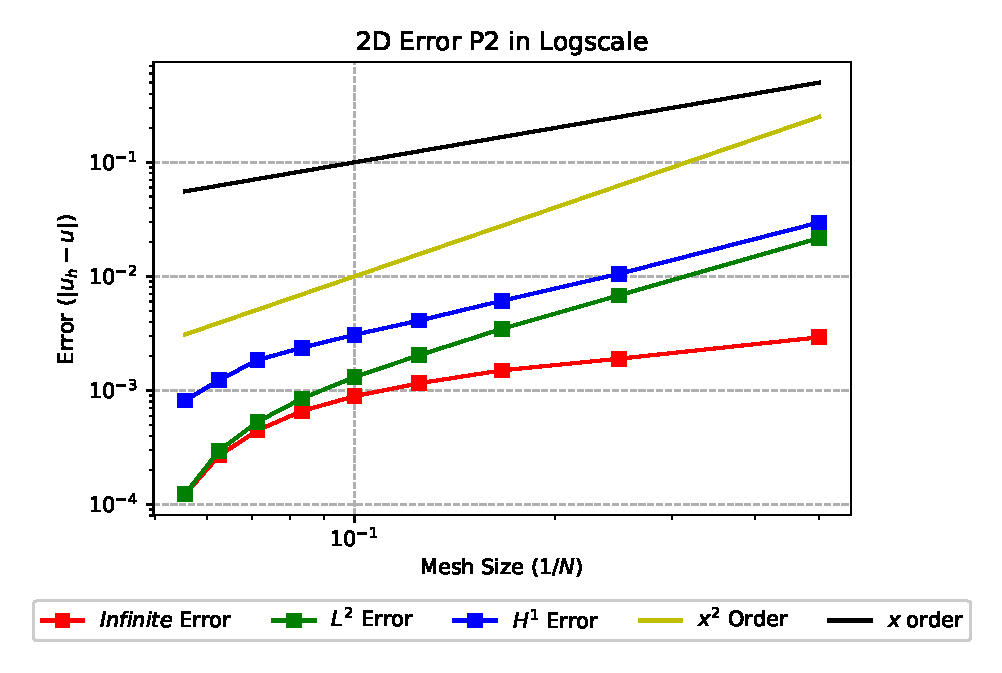
\includegraphics[width=\linewidth]{picture/conference/all2derrorP2}
		\caption{2D Error P2 Plot in Logscale}
		\label{fig:2derrorP2}
	\end{subfigure}
	\begin{subfigure}[b]{0.5\linewidth}
		\centering
		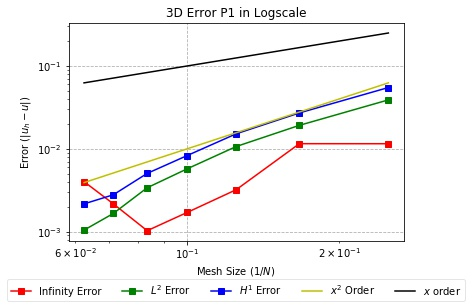
\includegraphics[width=\linewidth]{picture/conference/all3derrorP1}
		\caption{3D Error P1 Plot in Logscale}
		\label{fig:3derrorP1}
	\end{subfigure}
	\quad
	\begin{subfigure}[b]{0.5\linewidth}
		\centering
		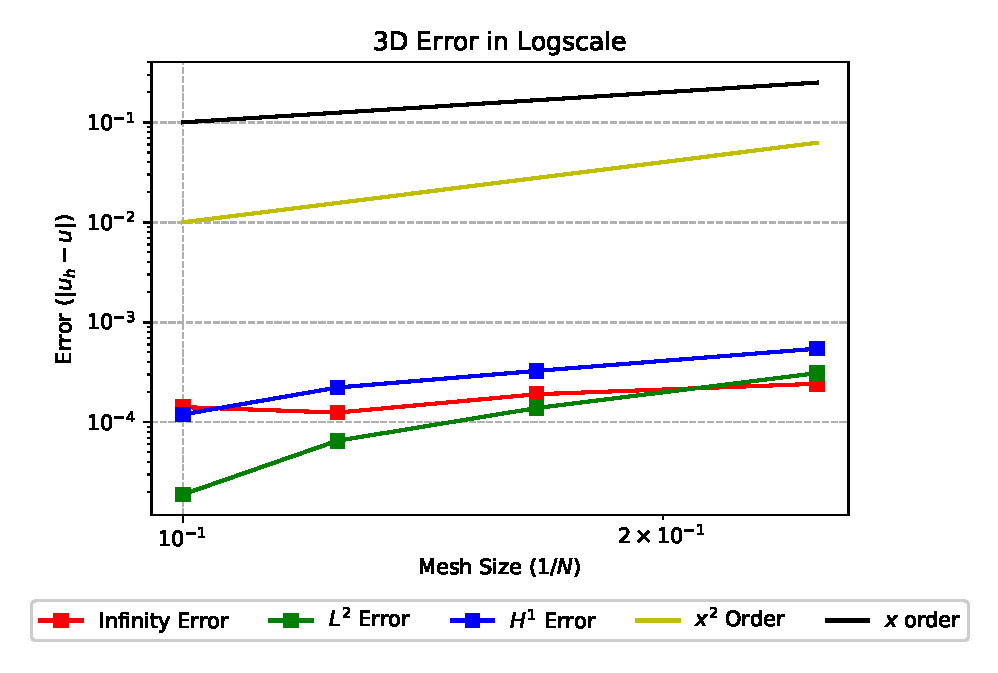
\includegraphics[width=\linewidth]{picture/conference/all3derror}
		\caption{3D Error P2 Plot in Logscale}
		\label{fig:3derrorP2}
	\end{subfigure}
	\caption{Error Plot in Logscale}
	\label{fig:errorplot}
\end{figure}

\newpage
\section{Linear Elasticity with Crack Propagation}
We solved problem \eqref{eq:weakcrack} using same model as shown in figure \ref{fig:3dmodel} and numerical parameter like in table \ref{tab:parametertable}, the difference from linear elasticity problem is the domain. In the crack propagation case, we disturb the domain with adding some so called "crack path" into the domain. For this case, we use n(division number) = 32 and d(width of the crack) = 0.001 [m]. The result of our simulation shown the figure \ref{fig:crackmodel} for 2D case:
\begin{figure}[h!]
	\begin{subfigure}[b]{0.5\linewidth}
		\centering
		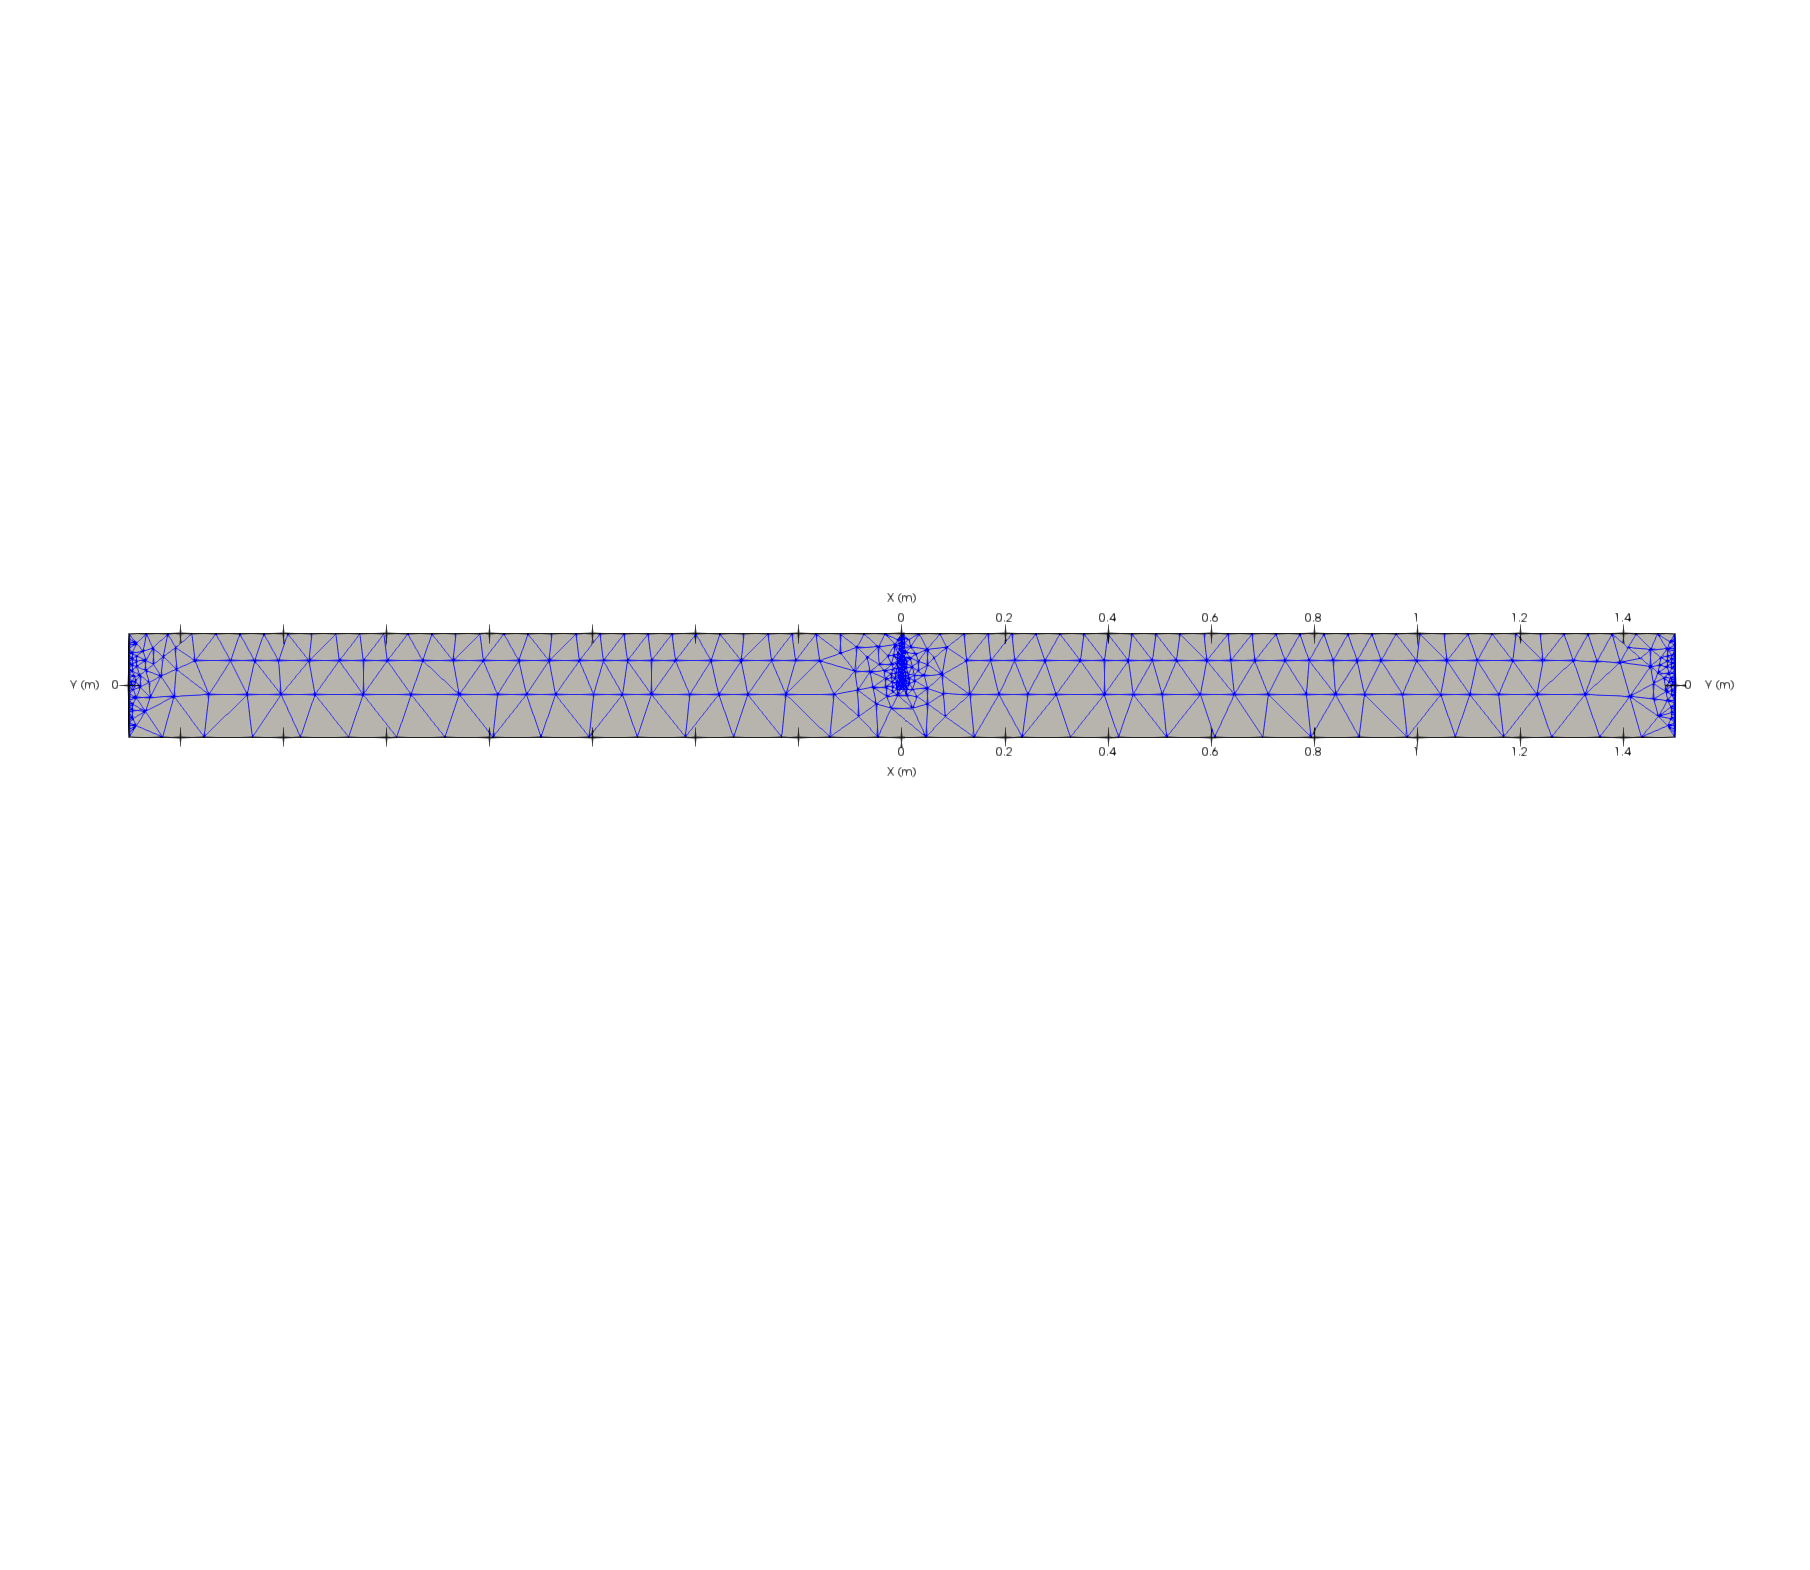
\includegraphics[width=\linewidth]{picture/conference/crackmodel2d}
		\caption{Elasticity with Crack Propagation Model in 2D}
		\label{fig:2dcrack}
	\end{subfigure}
	\quad
	\begin{subfigure}[b]{0.5\linewidth}
		\centering
		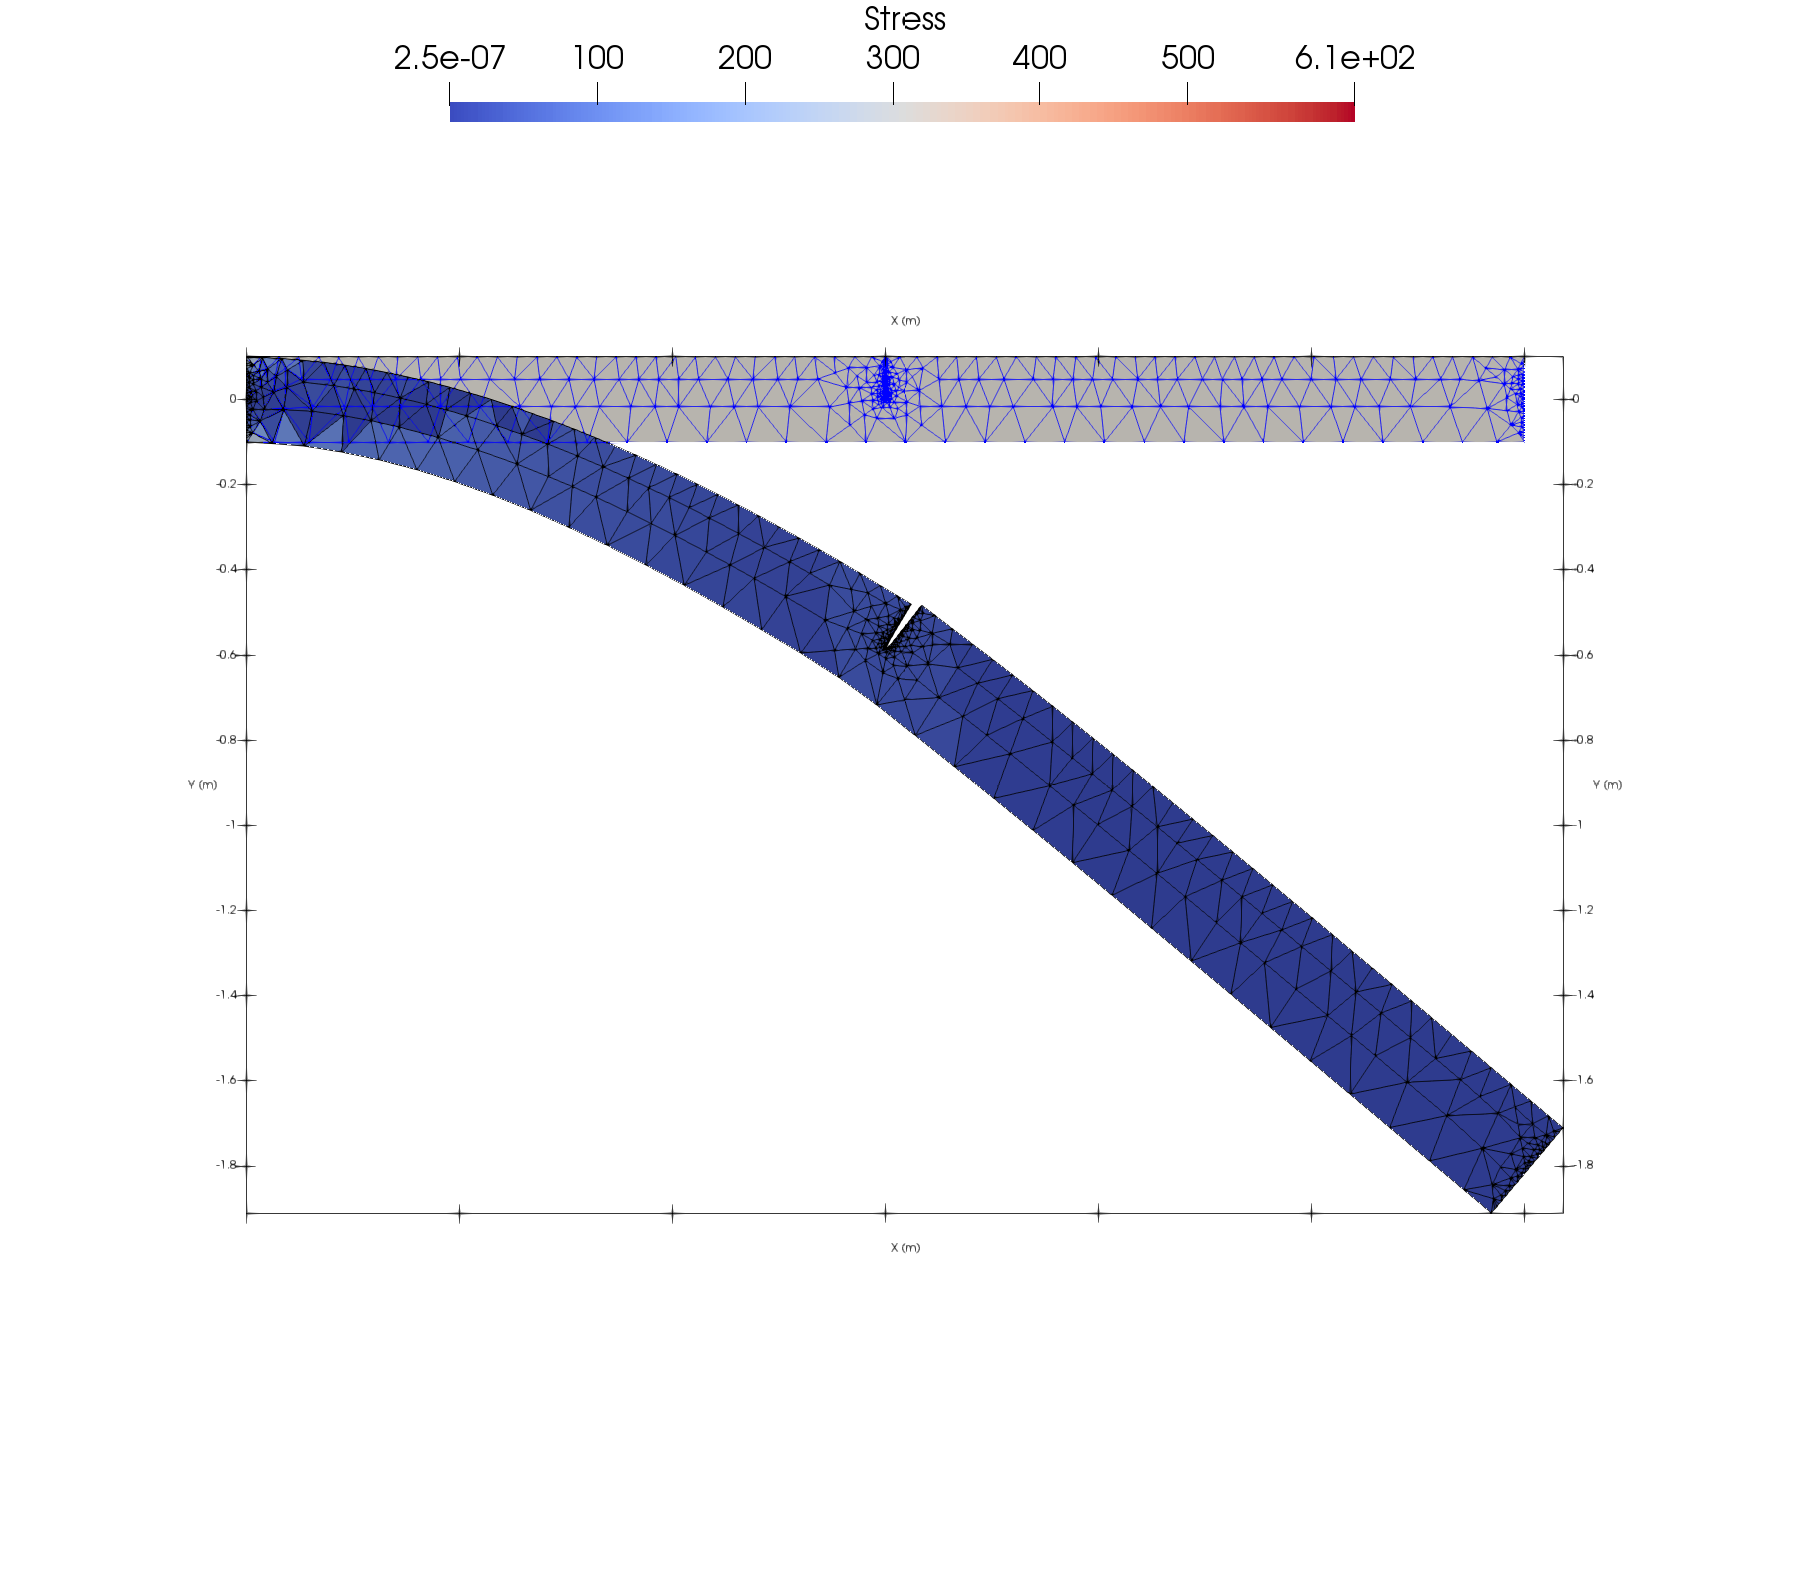
\includegraphics[width=\linewidth]{picture/conference/cracksol2d}
		\caption{Deformation of the material in Crack Propagation Case on 2D}
		\label{fig:2dcrackfinal}
	\end{subfigure}
	\quad
	\begin{subfigure}[b]{0.5\linewidth}
		\centering
		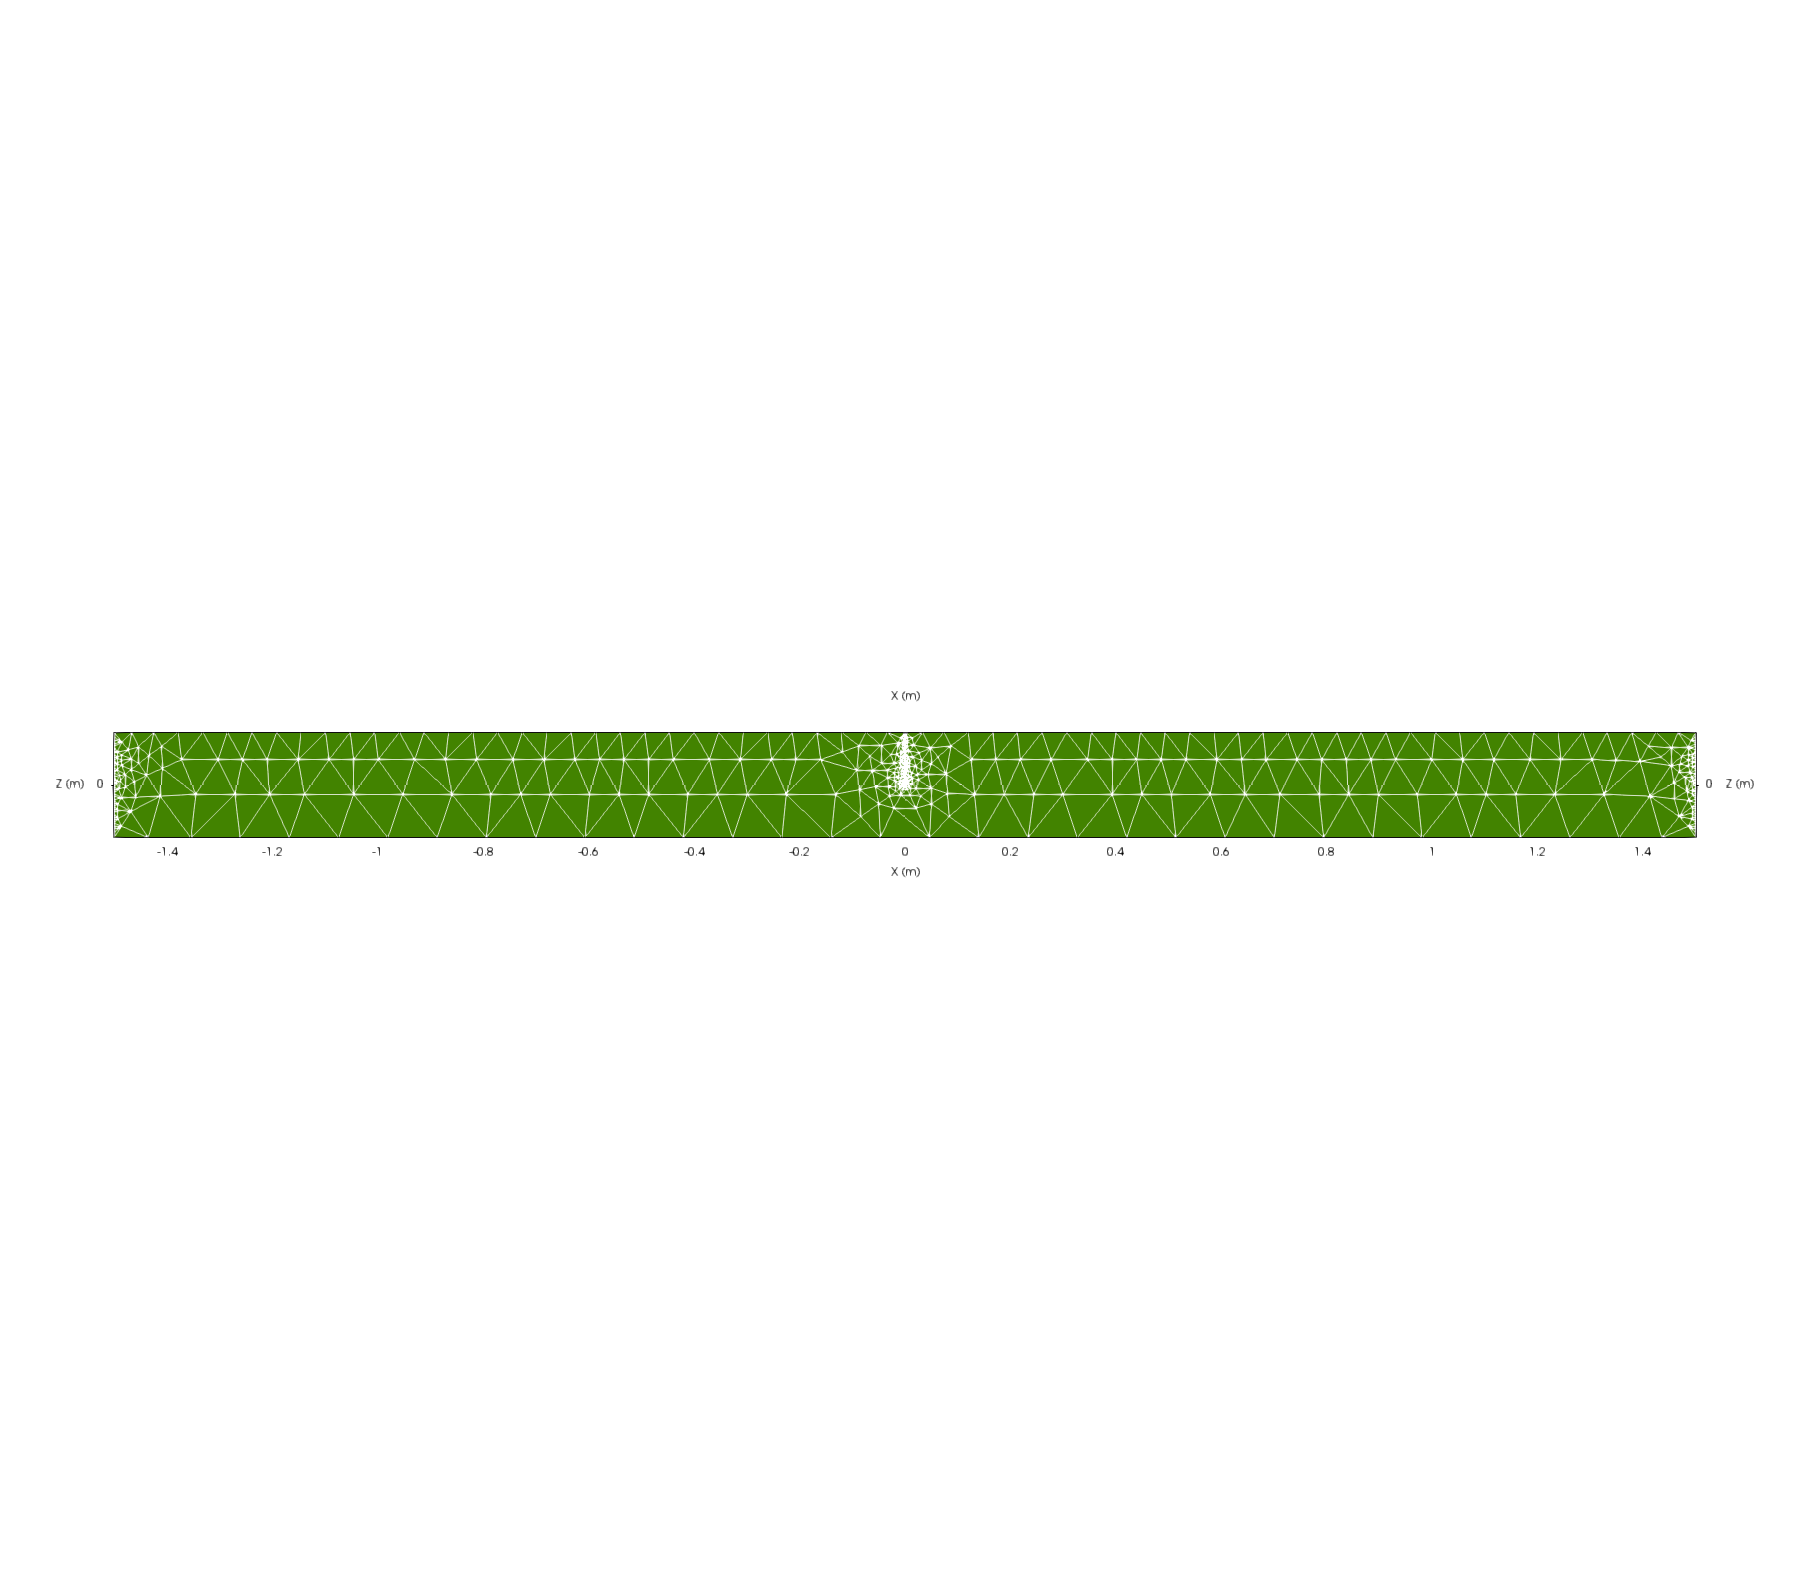
\includegraphics[width=\linewidth]{picture/conference/crackmodel3d}
		\caption{Elasticity with Crack Propagation Model in 3D}
		\label{fig:3dcrack}
	\end{subfigure}
	\quad
	\begin{subfigure}[b]{0.5\linewidth}
		\centering
		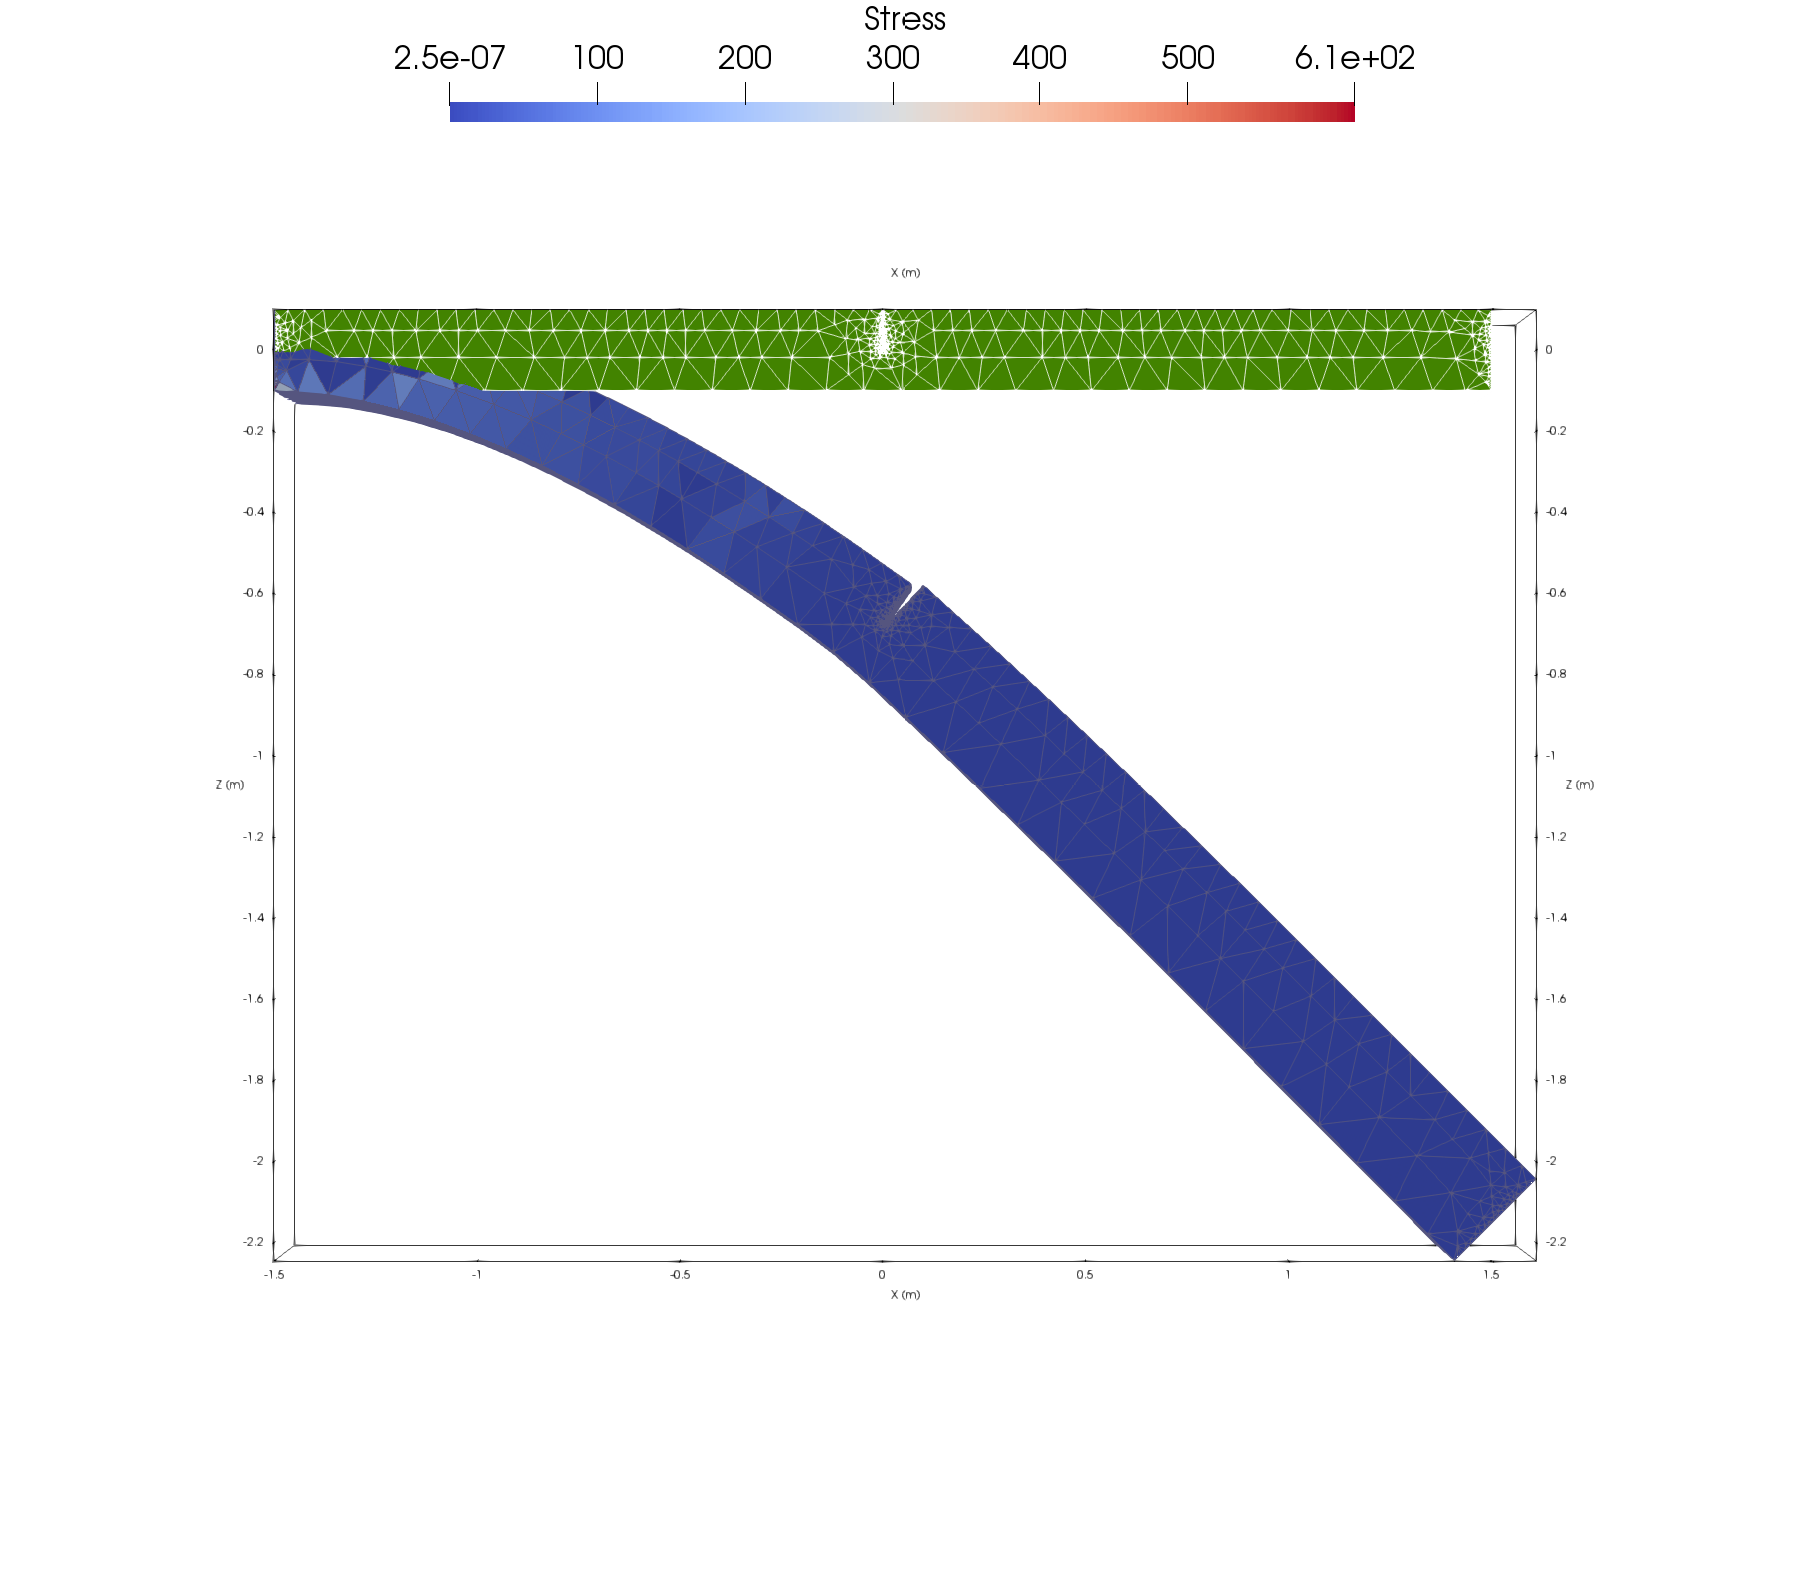
\includegraphics[width=\linewidth]{picture/conference/cracksol3d}
		\caption{Deformation of the material in Crack Propagation Case on 3D}
		\label{fig:3dcrackfinal}
	\end{subfigure}
	\caption{Elasticity with Crack Propagation Case in 2D and 3D}
	\label{fig:crackmodel}
\end{figure}\\
\newpage
After that, we also compare our 2D and 3D model in crack propagation case, the result is shown in the figure \ref{fig:compelast}\\
\begin{figure}[h!]
	\begin{subfigure}[b]{0.5\linewidth}
		\centering
		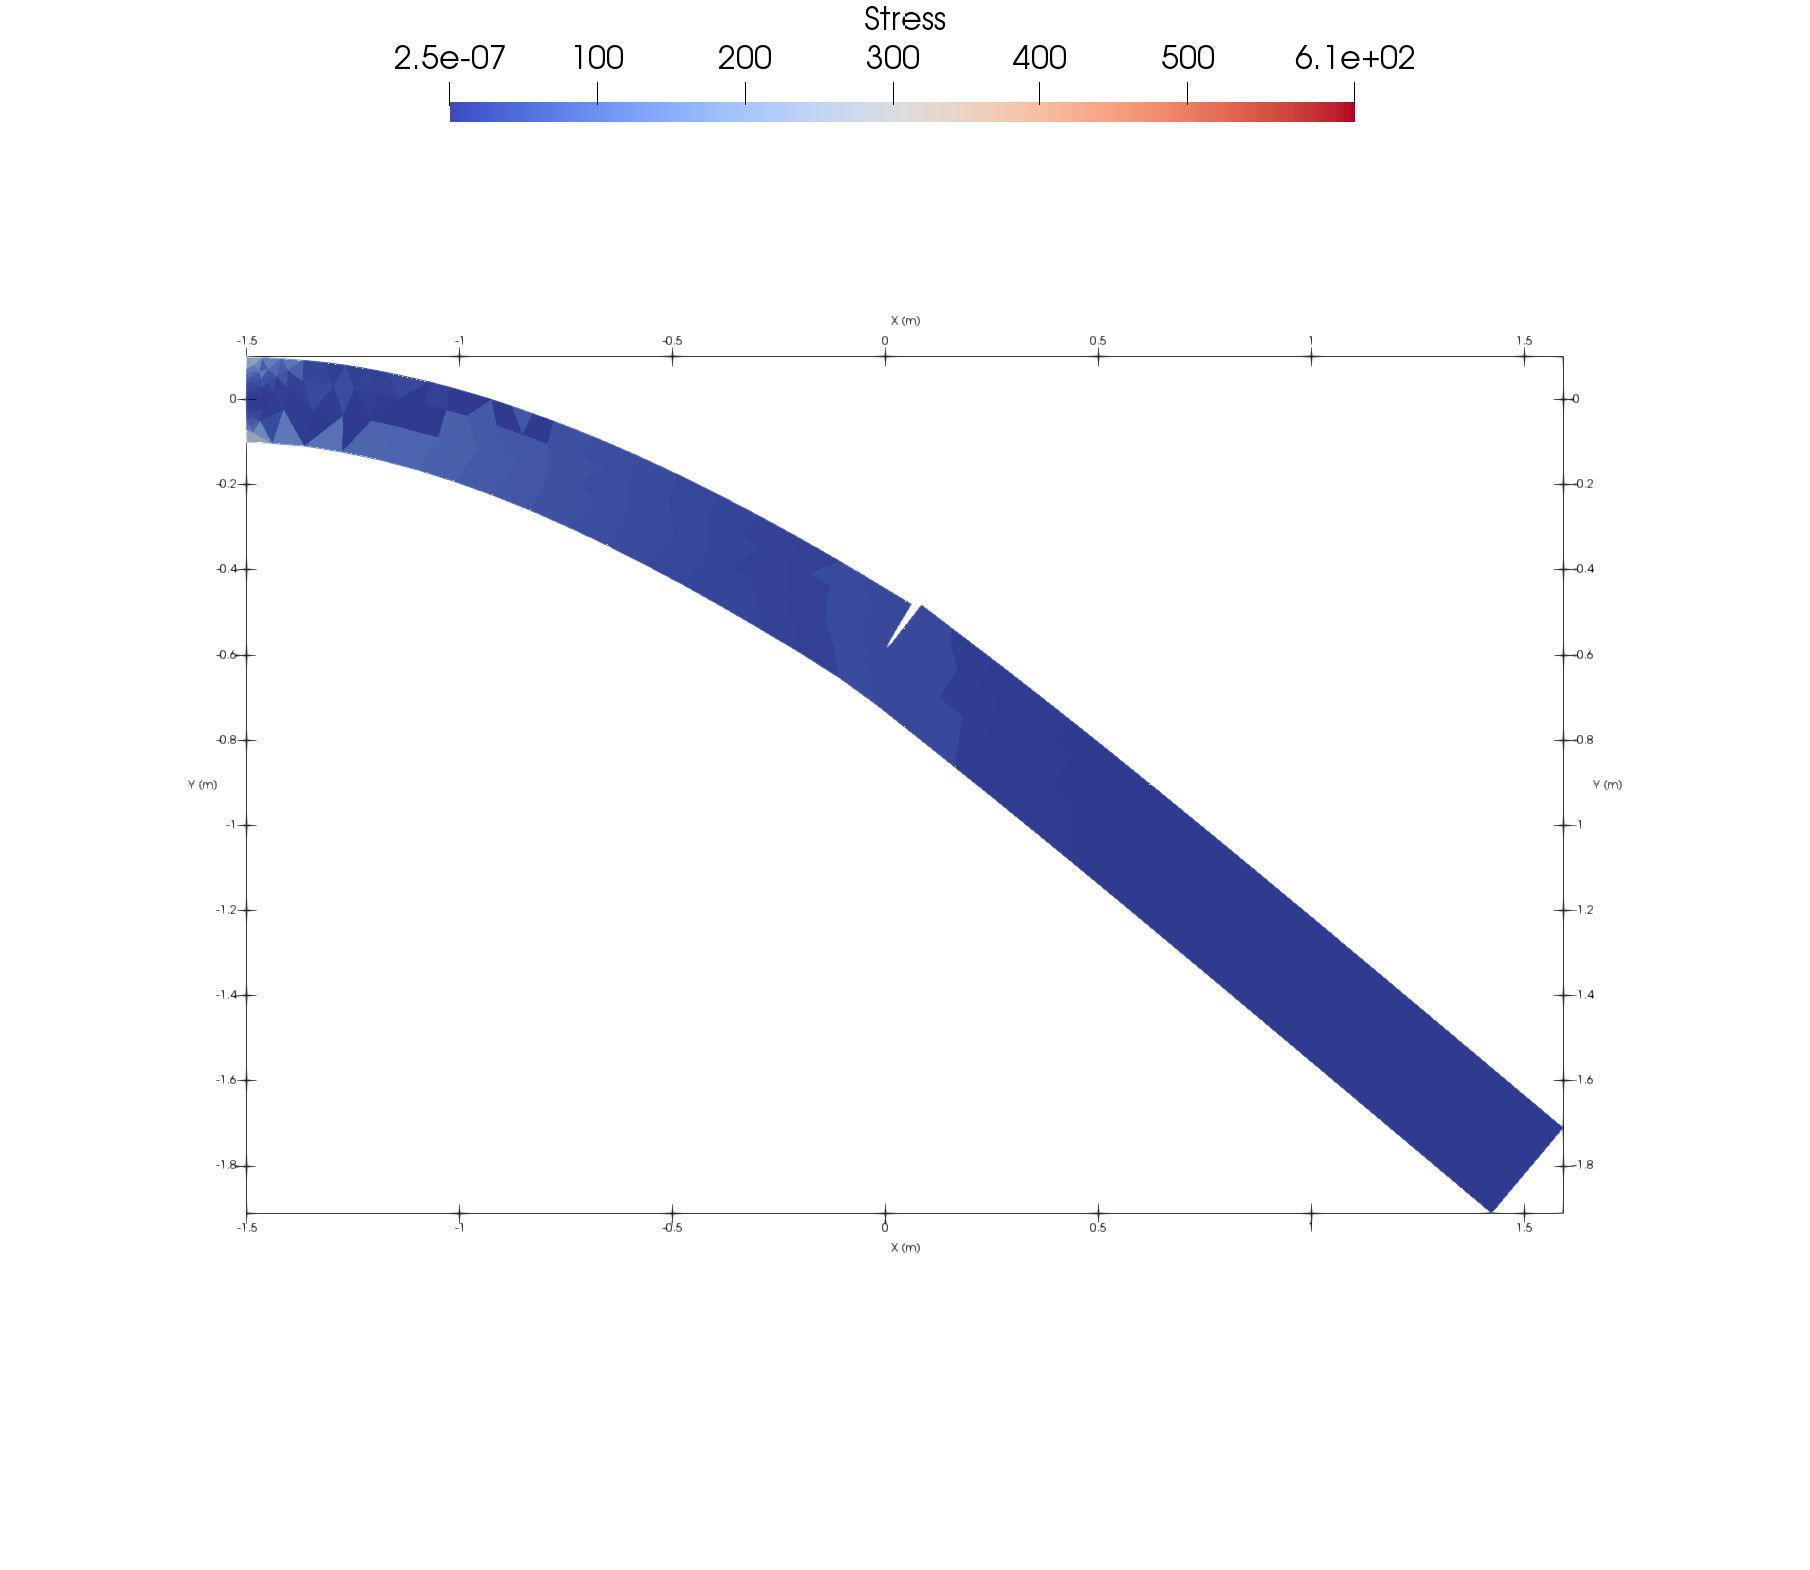
\includegraphics[width=\linewidth]{picture/conference/compare2d}
		\caption{Solution in 2D}
		\label{fig:2dcomp}
	\end{subfigure}
	\quad
	\begin{subfigure}[b]{0.5\linewidth}
		\centering
		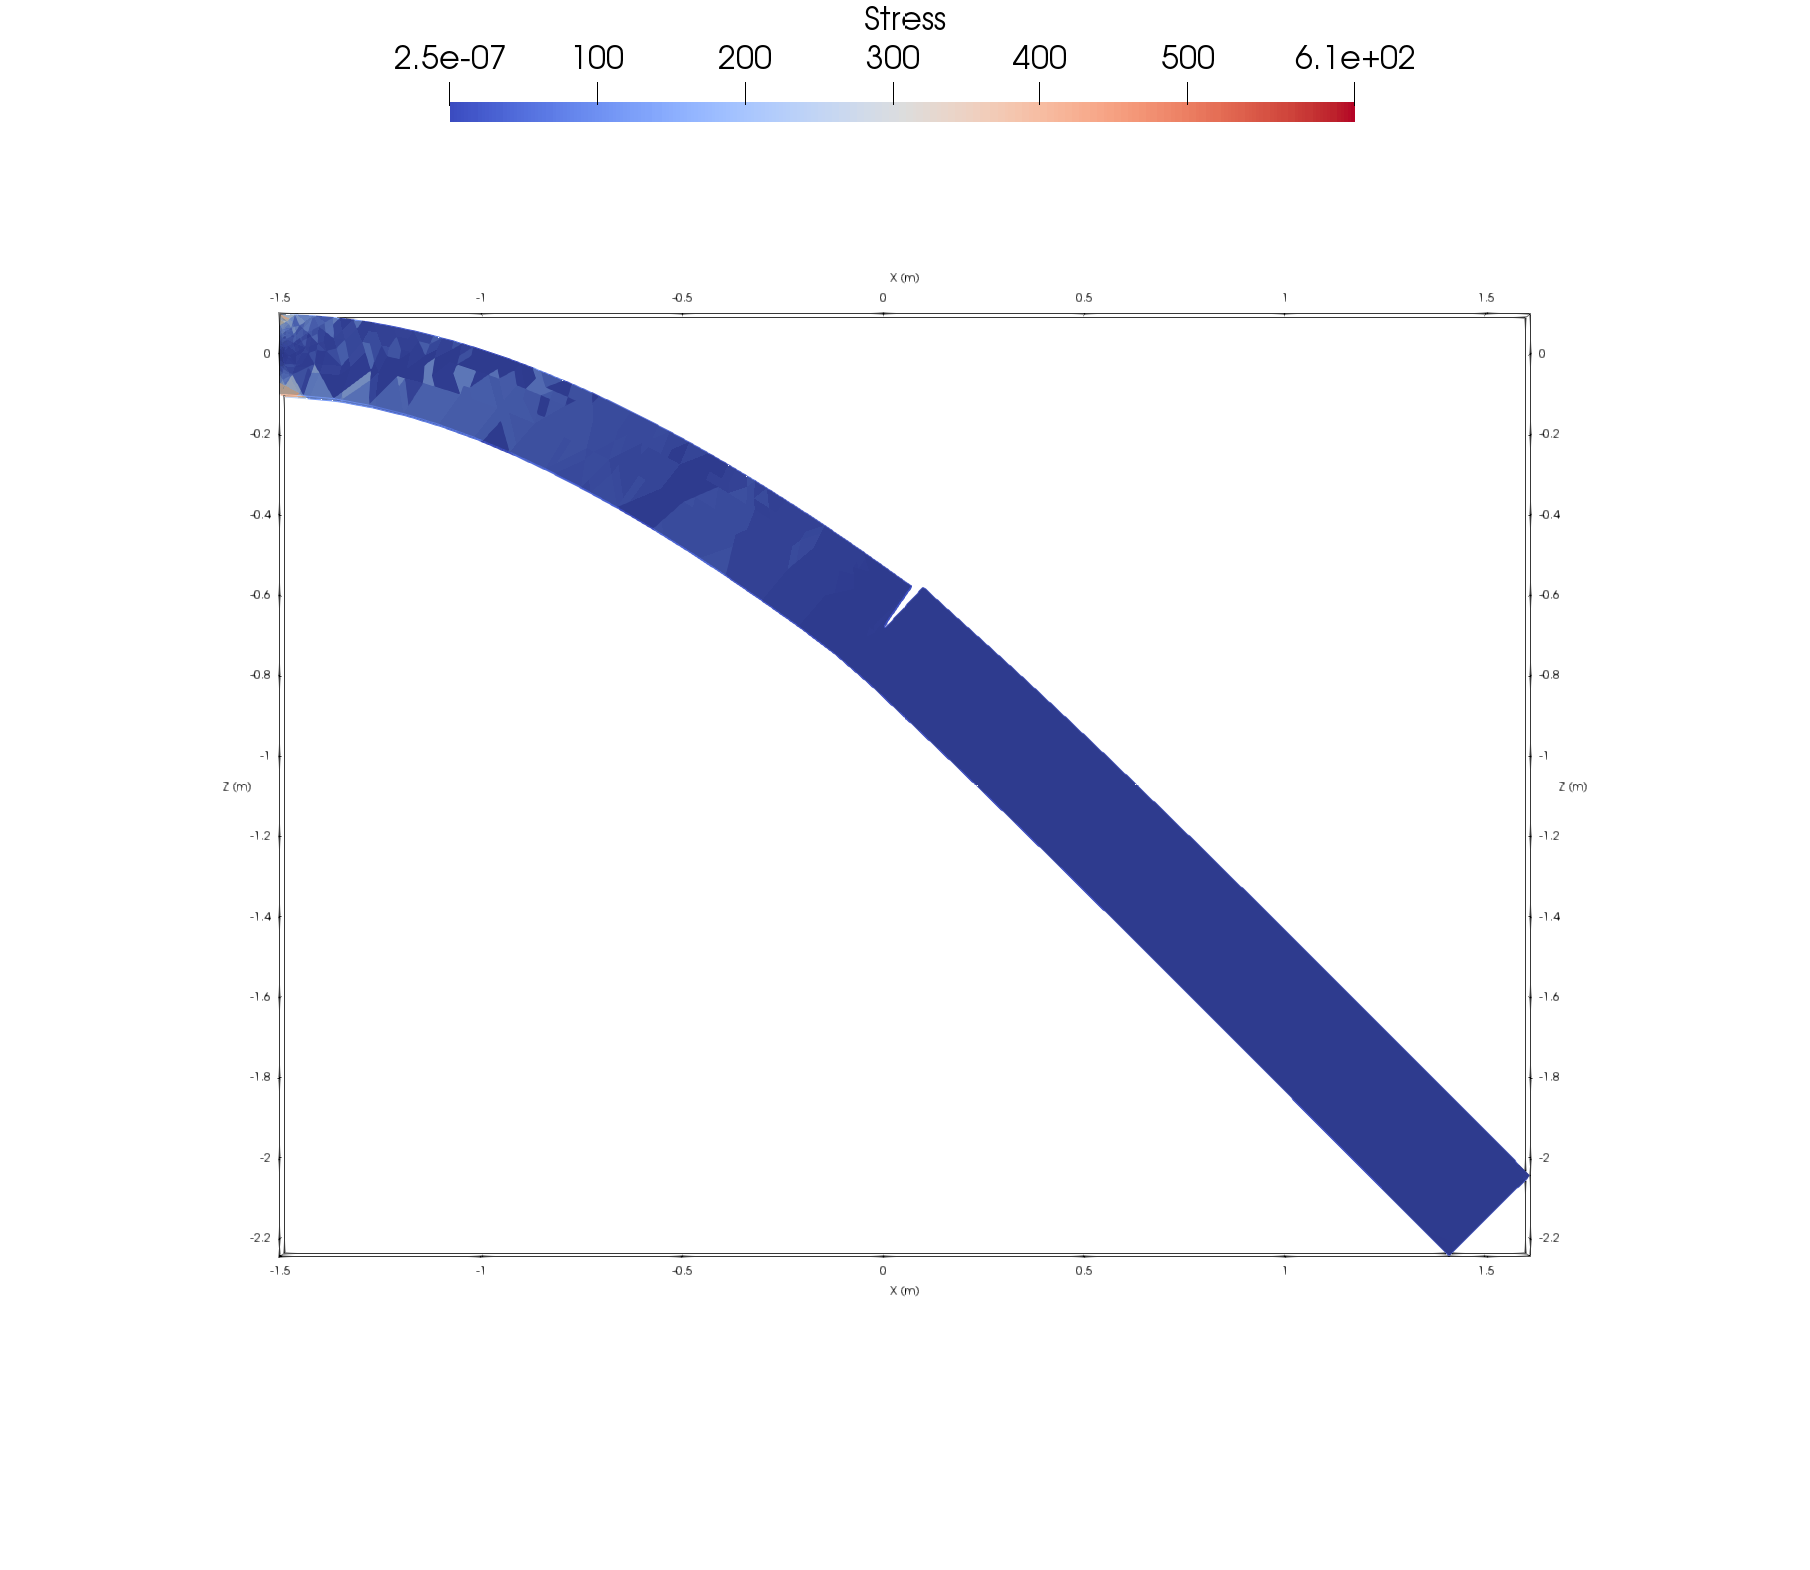
\includegraphics[width=\linewidth]{picture/conference/compare3d}
		\caption{Solution in 3D}
		\label{fig:3dcomp}
	\end{subfigure}
	\caption{Elasticity with Crack Propagation Case in 2D and 3D}
	\label{fig:compelast}
\end{figure}
\newline
We also calculated the elastic energy using equation \eqref{eq:elasticen}, below is the result of the energy profile from our model in figure \ref{fig:crackmodel}.
\begin{figure}[h!]
	\centering
	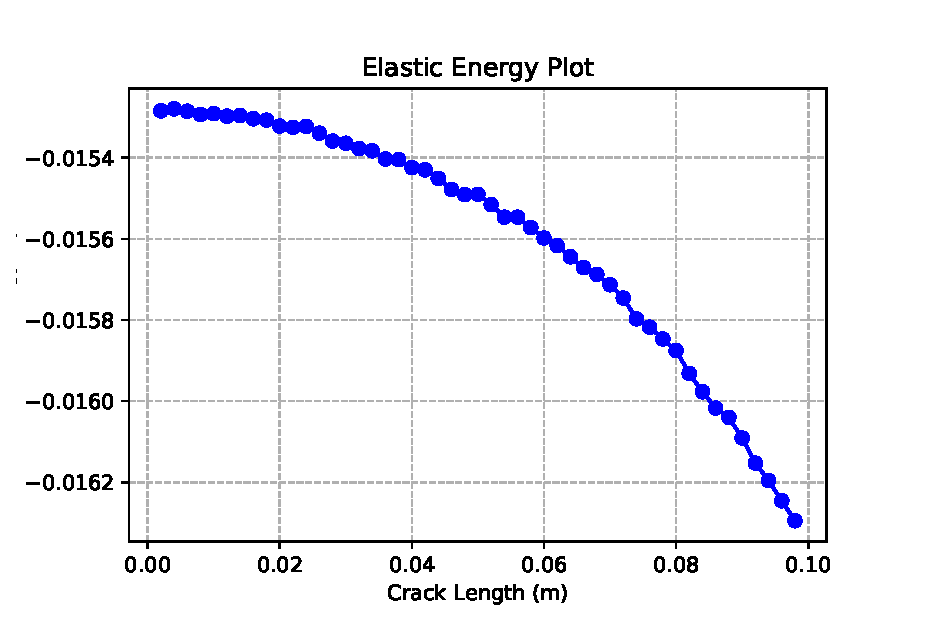
\includegraphics[width=0.8\linewidth]{picture/conference/elastic}
	\caption{Elasticity Energy Profile Crack Problem Model in 2D}
	\label{fig:elasticenergy}
\end{figure}
\end{document}